\documentclass[10pt,a4paper]{article}
\usepackage[margin=22mm]{geometry}
\usepackage{graphicx,booktabs,longtable,array,amsmath,amssymb,xurl,hyperref}
\usepackage[numbers,sort&compress]{natbib}
\providecommand{\bibcommenthead}{}
\hypersetup{hidelinks}
\renewcommand{\thetable}{S\arabic{table}}
\renewcommand{\thefigure}{S\arabic{figure}}
\emergencystretch=2em
\newcommand{\PopTwenty}{1.665}
\newcommand{\BuiltTwenty}{197.5}
\newcommand{\PopPctTwenty}{7.40}
\newcommand{\PopThirty}{3.020}
\newcommand{\BuiltThirty}{325.6}
\newcommand{\PopPctThirty}{13.42}
\newcommand{\PopForty}{4.891}
\newcommand{\BuiltForty}{464.6}
\newcommand{\PopPctForty}{21.74}
\newcommand{\PopTotal}{22.501}
\newcommand{\BuiltTotal}{1253.6}
\newcommand{\UniformOneMin}{4.763}
\newcommand{\UniformBiasMin}{57.7}
\newcommand{\UniformOneMax}{4.770}
\newcommand{\UniformBiasMax}{57.9}
\newcommand{\GHSLJointPct}{13.37}
\newcommand{\GHSLJointCommon}{2.989}
\newcommand{\WPJointPct}{23.20}
\newcommand{\WPJointCommon}{5.186}
\newcommand{\EpochOldPct}{20.86}
\newcommand{\EpochOldCommon}{4.664}
\newcommand{\EpochNewPct}{20.28}
\newcommand{\EpochNewCommon}{4.534}
\newcommand{\JointExcluded}{142.9}
\newcommand{\SampleTwentyEight}{3.051}
\newcommand{\SampleFiftySix}{3.232}
\newcommand{\SampleOneTwelve}{3.369}
\newcommand{\SampleTwoTwentyFour}{3.301}
\newcommand{\DWRTotal}{598098}
\newcommand{\DWRUnsupported}{1710}
\newcommand{\DWRSupportPct}{99.71}
\newcommand{\DWRUniformMin}{9022}
\newcommand{\DWRUniformMax}{9556}

\newcommand{\InteriorPopulationMin}{99.27}
\newcommand{\InteriorPopulationMax}{99.49}
\newcommand{\InteriorBiasMin}{58.24}
\newcommand{\InteriorBiasMax}{58.56}
\newcommand{\InteriorErrorMin}{98.55}
\newcommand{\InteriorErrorMax}{98.87}

\title{Supplementary Information\\Quantifying how spatial allocation and sampling alter population-weighted InSAR support summaries}
\author{Zixuan Liu and Wei Xiong}
\date{}
\begin{document}\maketitle
\section*{S1. Frozen domains and source provenance}
The authoritative experiment configuration is \texttt{config.json}. The primary domain consists of GHSL 3-arc-second pixels whose centers fall in the frozen finite footprint of the archived Chao Phraya VLM cells. Pixel rows in experiment NPZ files increase from south to north; GDAL raster rows and LiCSBAS binary files increase from north to south. Scripts explicitly convert between these conventions. No velocity-unit assumption enters the primary domain.

\begin{longtable}{p{.23\linewidth}p{.31\linewidth}p{.38\linewidth}}
\caption{Main input products and the information they provide.}\\
\toprule Product & Version/selection & Role and interpretation\\\midrule\endfirsthead
\toprule Product & Version/selection & Role and interpretation\\\midrule\endhead
Chao Phraya VLM & Zenodo 18092985, v2; public 1-km GeoTIFF & Frozen finite geographic footprint; WabInSAR source. Archived $\times10$ screen is supplementary and not independently established by raster unit tags.\\
LiCSAR & Frame 062D\_07629\_131313; 28 legacy pairs and 224 expanded pairs, 2016--2022 & Pairwise coherence and valid-unwrapped support diagnostics, not WabInSAR validity.\\
LiCSAR matched stack & Both dates in 2019--2020, baseline $\leq96$ days; 437 catalogue pairs & Separate small-area LiCSBAS processing and date-selected edge holdout.\\
GHSL & R2023A, GHS-POP and GHS-BUILT-S, 2020, 3 arcsec; 2015/2020, 30 arcsec & Extensive population and built-surface allocation models. Pixel scale is not independent demographic precision.\\
WorldPop & Thailand 2020, unconstrained UN-adjusted, 3 arcsec, record 29165 & Alternative count distribution. Common-total results isolate placement differences conditional on common validity.\\
ESA WorldCover & 2021 v200, tile N12E099, 10 m & Fractional cover strata within GHSL pixels; not a 2020 occupancy map.\\
DWR & Vertical Displacement Point Data Locations 2026Q1, layer 0 & Despite the service name, its geometry is polygons. Use actual measurement-cell union, not interpolation or arbitrary point buffers.\\\bottomrule
\end{longtable}

Source file URLs, hashes, geometries and download records are retained under \texttt{external/}, \texttt{results/fine/} and \texttt{results/lineage/}. The DWR fixed rectangle is selected before support results are computed. Its 38,738 polygons have 38,738 unique source codes. Their clipped-area sum and union agree to about $7\times10^{-5}$ m$^2$ (floating-point roundoff), confirming that repeated source cells do not inflate assigned population. The union area is 388.905 km$^2$ within a 495.510-km$^2$ domain.

\section*{S2. Historical lineage and non-equivalent statistics}
The submission-ready and staged submission-ready cell tables have the same SHA-256, \path{96ea01a6233315e8c37f06c55a5f0dac3656ae70239fded6b90aa68a63982a8a}. Both reproduce 12,589 selected legacy cells, population 3,772,492.0508 and built surface 404.772254 km$^2$. The alternate closure branch has hash \path{a17161efe405c98d01a221a549ee9e33a8cc3950a290d36c9a1f0b71ced68429} and yields zero cells under the same tabulated selection rule. This conflict is not evidence that the submitted arithmetic is unreproducible.

The legacy total sums whole-cell population selected by a center-majority rule. Point registration, unwrapped validity, support-statistic choice and population allocation change different parts of that calculation; they are not additive corrections to a validated physical exposure count. The revised mean area--pair deficit uses an explicitly different estimand.

The following factorial comparison holds archived cell centers and exposure weights fixed. The ``raw byte'' cutoff of 0.3 is intentionally retained only to diagnose incorrect encoding. GDAL point registration and added unwrapped validity are changed independently. These conditional legacy results must not be substituted for primary geographic-domain means.
\begin{table}[htbp]\centering\small
\caption{Binary center-majority lineage audit under the inherited strong screen. Population is in millions of full-cell allocation units.}
\begin{tabular}{lllrr}\toprule
Coherence encoding & Registration & Joint validity & Selected cells & Population\\\midrule
Raw byte (incorrect) & Legacy tiepoint & No & 0 & 0.000000 \\
Raw byte (incorrect) & Legacy tiepoint & Yes & 822 & 0.133146 \\
Raw byte (incorrect) & GDAL point & No & 0 & 0.000000 \\
Raw byte (incorrect) & GDAL point & Yes & 822 & 0.133819 \\
Byte / 255 & Legacy tiepoint & No & 12,589 & 3.772492 \\
Byte / 255 & Legacy tiepoint & Yes & 12,644 & 3.834586 \\
Byte / 255 & GDAL point & No & 12,582 & 3.756674 \\
Byte / 255 & GDAL point & Yes & 12,607 & 3.797393 \\
\bottomrule\end{tabular}

\end{table}

The full CSV additionally reports continuous center-frequency deficits for each combination and both domains. A center-majority rule, mean within-pixel area--pair support, and the fraction of area reaching a specified pass-count threshold are different statistics. For example, spatially uniform frequency 0.5 and a half-area split between frequencies 0 and 1 have the same mean, but different fractions meeting a frequency threshold of 0.5. Threshold distributions in this study refer to mean support at the GHSL grid, not an unobserved infinitely fine persistence distribution.

The VLM file has SHA-256 \path{5393e5c865c5105705b4b0e915f9133591816933965c88b67dfd273db6f2603d}. It contains no explicit stored-velocity unit tag. In the 18,077 frozen cells, directly applying a numerical cutoff of $-5$ to raw values selects no cells; applying it after the inherited multiplication by ten selects 17,808. This sensitivity explains why the primary experiments use a geographic domain. We neither establish that the conversion is wrong nor use agreement with an expected subsidence magnitude as proof that it is correct. The newer version 18093069 of the source repository contains random-forest code; it does not supply an explicit replacement unit record for this GeoTIFF.

\section*{S3. Geometry, conservation and numerical checks}
Coherence and unwrapped validity are intersected on the union of their actual raster boundaries before integration. A disjoint-mask analytical test confirms that their intersection is zero even if both separately averaged masks are one-half. Further tests cover extensive mass splitting, partial target coverage, half-pixel offsets, valid zero coherence and spherical area conservation.

All 512 production scale/origin/exposure/domain/method combinations preserve the native reference and the appropriate extensive total within the stated numerical tolerance. In the baseline summaries, the largest relative error in $S_E+U_E=T_E$ is $1.99\times10^{-15}$. The largest absolute covariance-identity residual is $5.96\times10^{-8}$ in the corresponding exposure units. Positive-, negative- and zero-covariance analytical examples verify the sign convention independently of the raster implementation. The exact empirical weighted-distribution integral matches the direct population deficit at printed precision.

The UTM transfer uses GDAL sum resampling of extensive first and cross moments. It is an approximate nonlinear reprojection; it is not described as exact spherical polygon reprojection. Production 50-m transfers close their totals within $10^{-8}$ relative tolerance. Recomputing from native inputs at 25 m produces measured relative total drifts of $-1.66\times10^{-5}$ for area, $-2.06\times10^{-5}$ for supported area, $-4.11\times10^{-6}$ for population and $-3.28\times10^{-6}$ for supported population. These diagnostic fields are not renormalized. Their maximum combined effect on the 1-km uniform population estimate is $2.40\times10^{-6}$ of the AOI population, or 0.00024 percentage points. The diagnostic drift is reported separately from the production conservation result.

These checks verify implementation identities and numerical stability. They do not establish population accuracy, velocity accuracy or independence of model inputs. The machine-readable records are \path{results/numerical_checks.json}, \path{results/allocation/conservation.csv} and \path{integration_convergence.csv}.

\section*{S4. Artificial masking, error denominators and synthetic bounds}
Each region has 21,600 method/scale/origin outputs: four missingness mechanisms, three removal fractions, 100 repetitions, three coarse sizes, two origins and three allocation rules. The same mask is used for all methods within a repetition. Gaussian smoothing generates spatial masks; density-associated scores combine standardized log density with a spatial term. The fixed seed is 20260927. Removal fractions refer to available fine pixels, while the realized removed area fraction is saved separately. In Fresno the controlled reference domain is the original published observed footprint, including its fractional intersections with GHSL pixels.

\begin{table}[htbp]\centering\small
\caption{Bangkok masking at 30\% removal, 10-pixel cells and zero origin. Error is relative to known removed allocation. Ranges are conditional mask percentiles.}
\begin{tabular}{llrr}\toprule
Mechanism & Method & Mean error (\%) & 2.5th--97.5th (\%)\\\midrule
density negative & area uniform & 120.35 & [105.55, 134.61] \\
density negative & building weighted & 19.60 & [17.46, 22.28] \\
density negative & cell center & 102.97 & [86.96, 121.20] \\
density positive & area uniform & -14.17 & [-15.15, -13.03] \\
density positive & building weighted & -4.99 & [-5.52, -4.47] \\
density positive & cell center & -11.64 & [-13.98, -9.39] \\
random & area uniform & 0.04 & [-0.40, 0.44] \\
random & building weighted & 0.03 & [-0.24, 0.27] \\
random & cell center & 0.08 & [-9.19, 8.76] \\
spatial & area uniform & 0.01 & [-0.82, 0.81] \\
spatial & building weighted & 0.01 & [-0.50, 0.50] \\
spatial & cell center & 0.01 & [-3.60, 3.12] \\
\bottomrule\end{tabular}

\end{table}

When the removed population is small, relative errors can be large: low-density-associated removal at 10\% of pixels is such a case. Main-text Fig.~4 instead normalizes by the entire test-domain population, so a large ratio is not mistaken for a large fraction of all residents. Raw reference totals, estimates, signed errors, cell RMSE and absolute cell-error totals remain available for every scenario. Building-weighted improvement is conditional on GHSL's shared built-environment information and should not be generalized to independently observed household locations.

The synthetic hazard fields are experiment definitions, not inferred or measured deformation. With threshold membership $h_p\in\{0,1\}$ and introduced missingness $m_p$, the omitted threshold allocation $\sum_p E_p h_p m_p$ lies between zero and $\sum_p E_p m_p$. Adding observed threshold allocation gives the identification interval in the main text. All synthetic checks satisfy that deterministic bound. No probability coverage or external geodetic validation is claimed. Complete outputs are under \texttt{results/masking/} and \texttt{results/dwr/masking/}.

The Fresno repeat shows the same sign reversal with different magnitudes (Fig.~S4). At 30\% removal, 10-pixel cells and zero origin, uniform-area mean error is $-16.14$ percentage points of the observed-footprint population for high-density-associated removal and $+7.28$ points for low-density-associated removal. The corresponding built-weighted errors are $-10.61$ and $+4.23$ points. Uniform-area mean errors for random and unrelated spatial masks are $-0.021$ and $-0.0025$ points. Relative-to-removed-population errors can be very large in sparsely populated masks; both denominators are retained, and the figure uses the whole observed-footprint total. These results support a conditional allocation mechanism, not a universally successful correction.

\section*{S5. Expanded sampling and temporal network}
The catalogue snapshot contains 1,603 pairs with both dates in 2016--2022. The 224-pair pool comprises eight randomly ranked pairs from each of 28 year--quarter strata, alternating short ($\leq24$ days) and long baselines as availability permits. An amendment swapped adjacent ranks in even quarters before support outcomes were extracted. Both the original rank plan and amended plan are retained. This improved baseline balance but did not force equal counts where long-baseline availability was limited.

\begin{table}[htbp]\centering
\caption{Nested pool composition and population deficit at $q=0.3$.}
\begin{tabular}{rrrr}\toprule
Pairs & Short baseline & Long baseline & Deficit (millions)\\\midrule
28 & 16 & 12 & \SampleTwentyEight{}\\
56 & 30 & 26 & \SampleFiftySix{}\\
112 & 60 & 52 & \SampleOneTwelve{}\\
224 & 120 & 104 & \SampleTwoTwentyFour{}\\\bottomrule
\end{tabular}
\end{table}

The equal-pair mean describes this sample design, not a catalogue-frequency-weighted population parameter. Start-date season does not contain the full seasonal history of a long-baseline pair. The additional repeated samples draw 1, 2, 4 or 8 pairs per year--quarter without replacement from the fixed eight-pair stratum; their conditional distributions characterize design sensitivity. A 224-pair draw contains the entire fixed pool, so its variation is zero by construction, not proof of zero uncertainty. Shared acquisitions and atmospheric signals mean that individual pairs are not independent replicates of physical accuracy.

\begin{figure}[htbp]\centering
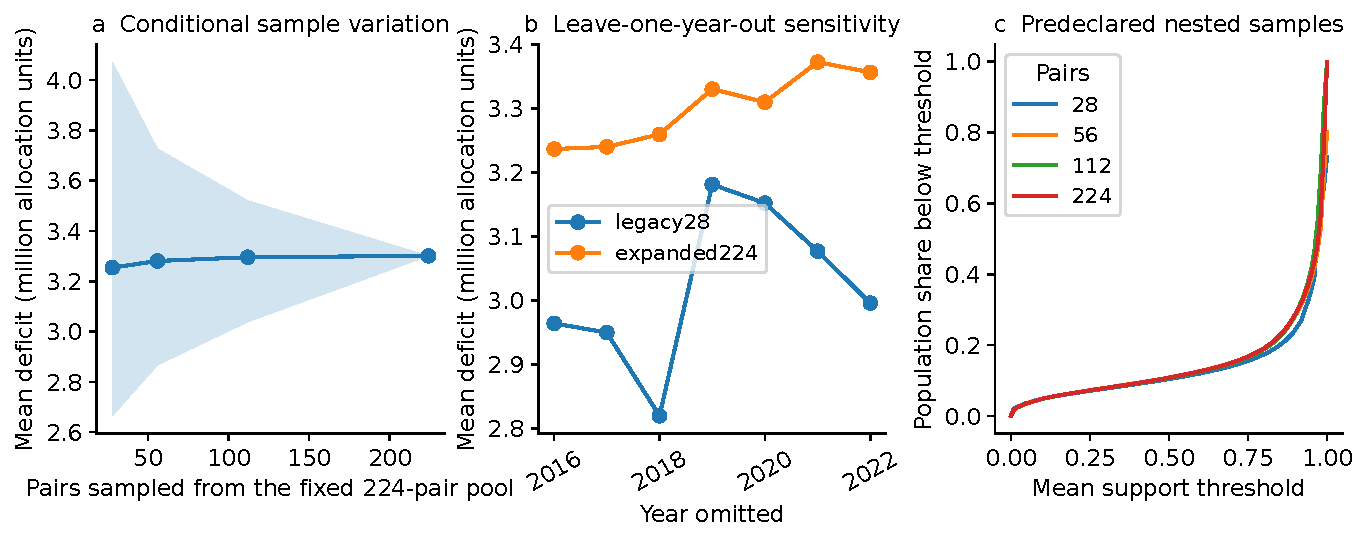
\includegraphics[width=\linewidth]{figures/S1_sampling.pdf}
\caption{Conditional sampling variation, leave-one-year-out sensitivity and support distributions from nested samples. Bands in the first panel are the central 95\% of introduced draws from the fixed pool; they are not confidence intervals for a complete time-series product.}\end{figure}

\begin{table}[htbp]\centering
\caption{Date-graph diagnostics; these do not establish pixel-level connectivity.}
\begin{tabular}{lrrrr}\toprule
Graph & Pairs & Dates & Components & Independent cycles\\\midrule
Legacy sample & 28 & 54 & 26 & 0\\
Expanded pool & 224 & 225 & 29 & 28\\
Catalogue 2016--2022 & 1603 & 288 & 1 & 1316\\\bottomrule
\end{tabular}
\end{table}

Native pixels are aggregated by center into fixed $0.05^\circ$ longitude--latitude blocks anchored at integer multiples of $0.05^\circ$. All blocks are retained in the CSV; rank comparisons use the 539 blocks with at least 1,000 GHSL population units and 5 km$^2$ inside the domain. Relative to the 224-pair pool, the nested 28-, 56- and 112-pair deficit-amount rank correlations are 0.9940, 0.9992 and 0.9994. Their top-decile Jaccard overlaps are 0.8000, 0.8621 and 0.9286. Deficit-share correlations exceed 0.9991. Thus similar overall ranks can coexist with changed totals and changed membership near a selection boundary. These comparisons describe sampling stability; they do not validate measurement priorities or make the 224-pair pool a true target. Spatial blocks are not treated as independent accuracy replicates.

\begin{figure}[htbp]\centering
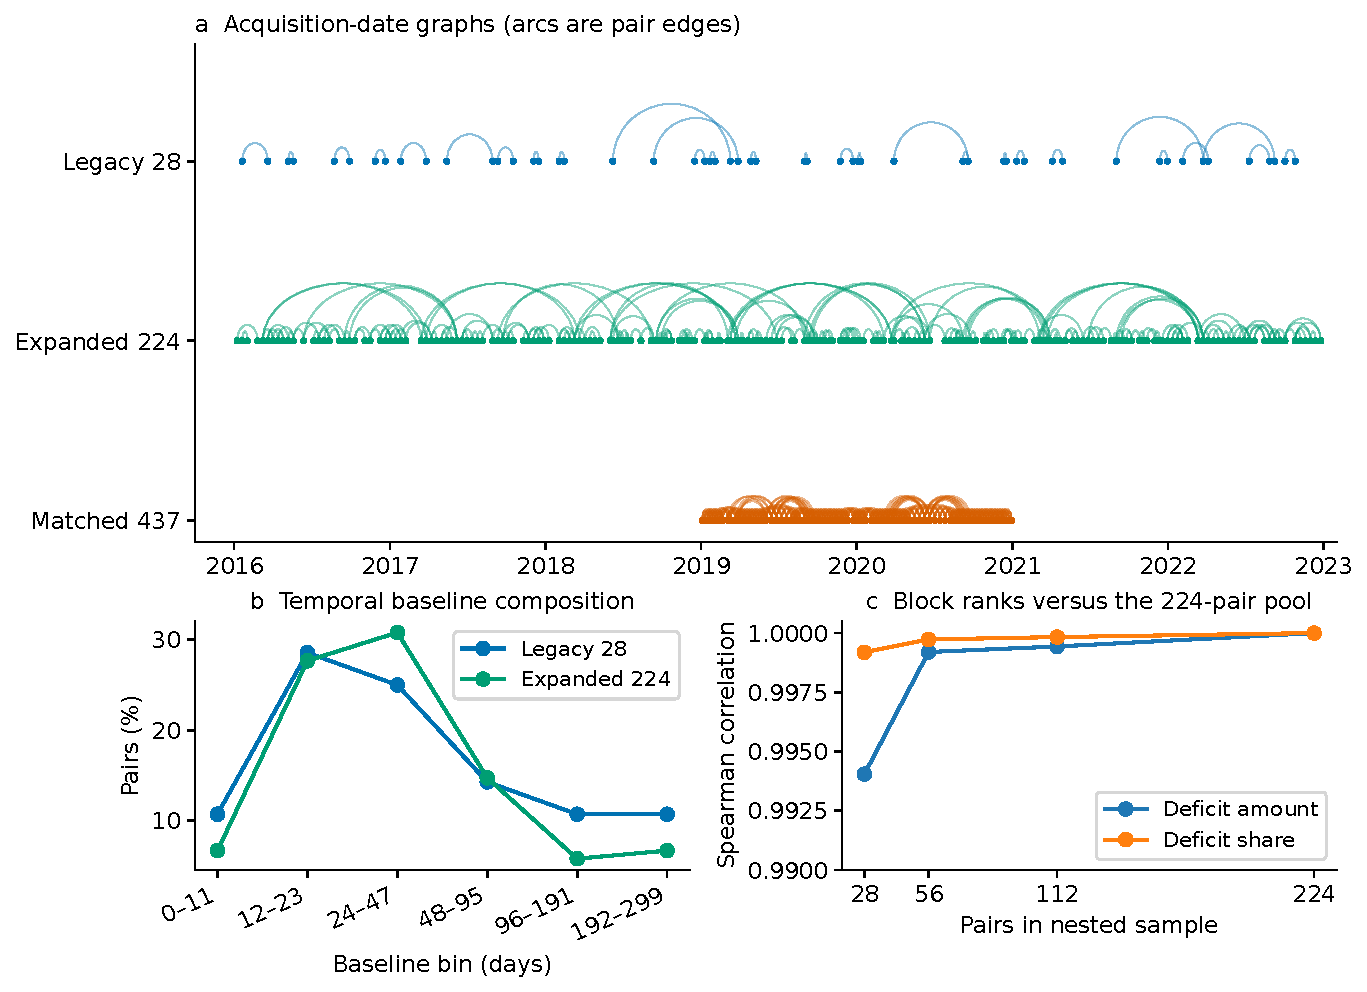
\includegraphics[width=\linewidth]{figures/S2_network_ranks.pdf}
\caption{Actual acquisition-date graphs, temporal-baseline composition and descriptive block-rank sensitivity. Each arc joins the two dates of an input pair; graph connectivity is reported in Table~S5. The matched graph precedes quality rejection. The rank panel uses a restricted vertical range to show small differences; all comparisons use the same 539 eligible blocks and the fixed 224-pair pool as comparator.}\end{figure}

\section*{S6. Population coverage and land-cover interpretation}
The main population-model comparison restricts to fine pixels covered to within $10^{-5}$ by all four compared model/epoch rasters. The common domain contains 1,754,190 fine pixels and excludes \JointExcluded{} thousand GHSL population units relative to the primary footprint. Outputs on each product's own valid coverage are retained alongside common-coverage outputs. NoData is not silently converted into a zero population for comparative denominators.

Normalization multiplies each population model by the same target total divided by its own common-domain total. Its weighted support share is consequently unchanged; this isolates spatial distribution from differences in population totals. The common-total q0.3 results are \GHSLJointCommon{} million for native GHSL and \WPJointCommon{} million for WorldPop. Neither establishes demographic truth. A difference between 2015 and 2020 GHSL at fixed 30 arcsec is an epoch/model sensitivity; comparing native 3-arcsecond 2020 to coarse 2015 alone would confound epoch and resolution.

All 11 ESA WorldCover class codes are processed by native fractional intersection. Their fractions sum to one inside the primary domain within $2\times10^{-5}$. Reported nonzero classes include built-up, tree cover, cropland, grassland, bare/sparse vegetation, permanent water, wetland, shrubland and mangroves. GHSL allocations within a mixed cover pixel remain uniform at the subpixel level. Classification uncertainty, mixed pixels and the 2021 epoch are not converted into a probabilistic population uncertainty estimate.

\section*{S7. Matched LiCSBAS processing and holdout}
The upstream LiCSBAS2 commit is \path{2627e50a1c703becd4a0b18754b05c1cf8c564d5}. Both branches complete steps 11--16 without changes to tracked scientific source. A documented Windows I/O wrapper substitutes a native parameter reader for external grep and copies browse PNGs instead of creating symlinks. Its optional GDAL import only affects unused GeoTIFF helper functions. Input preparation uses Rasterio independently. All processing is serial with a fixed NumPy seed; package versions and the exact wrapper diff are retained.

The canonical processing raster has 301 columns and 401 rows, with actual affine transform recorded in \path{results/timeseries/geometry.json}; its pixel spacing is approximately 108 by 111 m at this latitude. The input frame is 062D\_07629\_131313. Global input connectivity is a selection requirement, not a guarantee of pixel-level connectivity. Of 437 full-stack inputs, 431 survive pair-level checks; of 393 training inputs, 382 survive. Both original holdout membership and rejected-pair lists are saved. Held-out phase/coherence is never used by the training workflow.

Step 11 uses the upstream mean-coherence threshold 0.05 and unwrapped-coverage threshold 0.3. Step 12 uses a loop threshold of 1.5 rad. Step 13 uses least squares with regularization parameter 0.0001 and requires more than 104 valid interferograms for inversion. Step 14 retains the upstream 100 bootstrap draws and spatiotemporal-consistency calculation. Bootstrap velocity spread is a processing diagnostic, not a calibrated uncertainty interval for physical velocity.

Step 15 uses fixed C-band defaults with automatic threshold relaxation disabled: mean coherence at least 0.05, at least 156 valid interferograms, velocity spread at most 100 mm yr$^{-1}$, maximum connected duration at least one year, at most 10 temporal gaps, spatiotemporal inconsistency at most 5 mm, at most 50 interferograms without a loop, at most 5 loop errors and inversion residual RMS at most 2 mm. The combined mask therefore contains information beyond the $q=0.3$ input diagnostic. It also shares coherence information with that diagnostic. Rates in the saved mask logs use the upstream finite/non-reference denominator; reported domain fractions count all 120,701 processing cells and explicitly include the finite reference pixel.

Step 16 applies the upstream 2-km spatial and 21-day temporal filter, without detrending, DEM-error fitting or height-linear correction. Both filtered products are retained, but the held-out prediction is deliberately evaluated from \texttt{cum.h5}, the unfiltered training inversion. Thus prediction does not introduce a filtering-dependent smoothing comparison. No atmospheric correction or external GNSS datum is added. LOS displacement is relative and positive toward the satellite under the coefficient $-c/(4\pi f)$, with $f=5.405$ GHz; it is not converted to vertical motion.

For a held-out pair $(a,b)$, predicted displacement is the difference between training cumulative displacements at $b$ and $a$. Observed phase is converted to millimeters after subtracting its mean at the training reference area, \texttt{141:142/218:219}. The reference is selected entirely from training data. Held-out pairs missing a required training date or finite/nonzero phase at that reference are excluded explicitly. There are 44 evaluated and 0 excluded pairs. No spatial offset is fitted to minimize held-out errors. Prediction locations must have finite predicted displacement and valid nonzero held-out phase; low-coherence observed held-out values are not selectively discarded. Consequently these residuals include errors in the held-out observations as well as training predictions. Evaluability does not establish permanent-gap validity.

All-prediction pooled RMSE is 0.984 mm, versus 0.699/5.150 mm inside/outside the training quality mask. Training-only support bins range from 2.338 mm in the lowest group to 0.412 mm in the highest group. This comparison uses no held-out coherence in its strata. We additionally compare three predictions on identical evaluable observations: cumulative time-series differences, training HDF5 linear velocity multiplied by the pair interval in years (365.25 days), and zero relative displacement. Their pooled RMSE values are 0.984, 11.751 and 11.784 mm. The velocity baseline uses the same final training reference as the cumulative series. Neither baseline uses held-out measurements for fitting. All held-out acquisition dates remain represented in training: this tests edge reconstruction, not prediction at unseen dates. Reconstructed date-dependent atmospheric phase can contribute to the difference from a linear or zero-displacement baseline, so the improvement does not establish deformation accuracy. Shared dates and atmospheric components limit independence, so spatial-pixel sample sizes and pair counts are descriptive denominators, not effective independent sample sizes. Five support thresholds (0.2, 0.3, 0.5, 0.7, 0.8), all four confusion categories, population/area weights, support-bin counts and quality medians are saved rather than selecting only one favorable threshold.

Evidence files are \path{support_finalmask_confusion.csv}, \path{support_quality_bins.csv}, \path{heldout_pairs.csv}, \path{heldout_support_bins.csv}, \path{heldout_prediction_comparison.csv}, \path{descriptive_correlations.csv} and \path{audit.json} within \path{results/timeseries/}. The audit verifies all twelve stage completions, absence of held-out edges from training input directories, population conservation in confusion tables, pooled residual reconstruction and independent recomputation of selected pair residuals. It verifies implementation and design, not external physical accuracy.

\begin{figure}[htbp]\centering
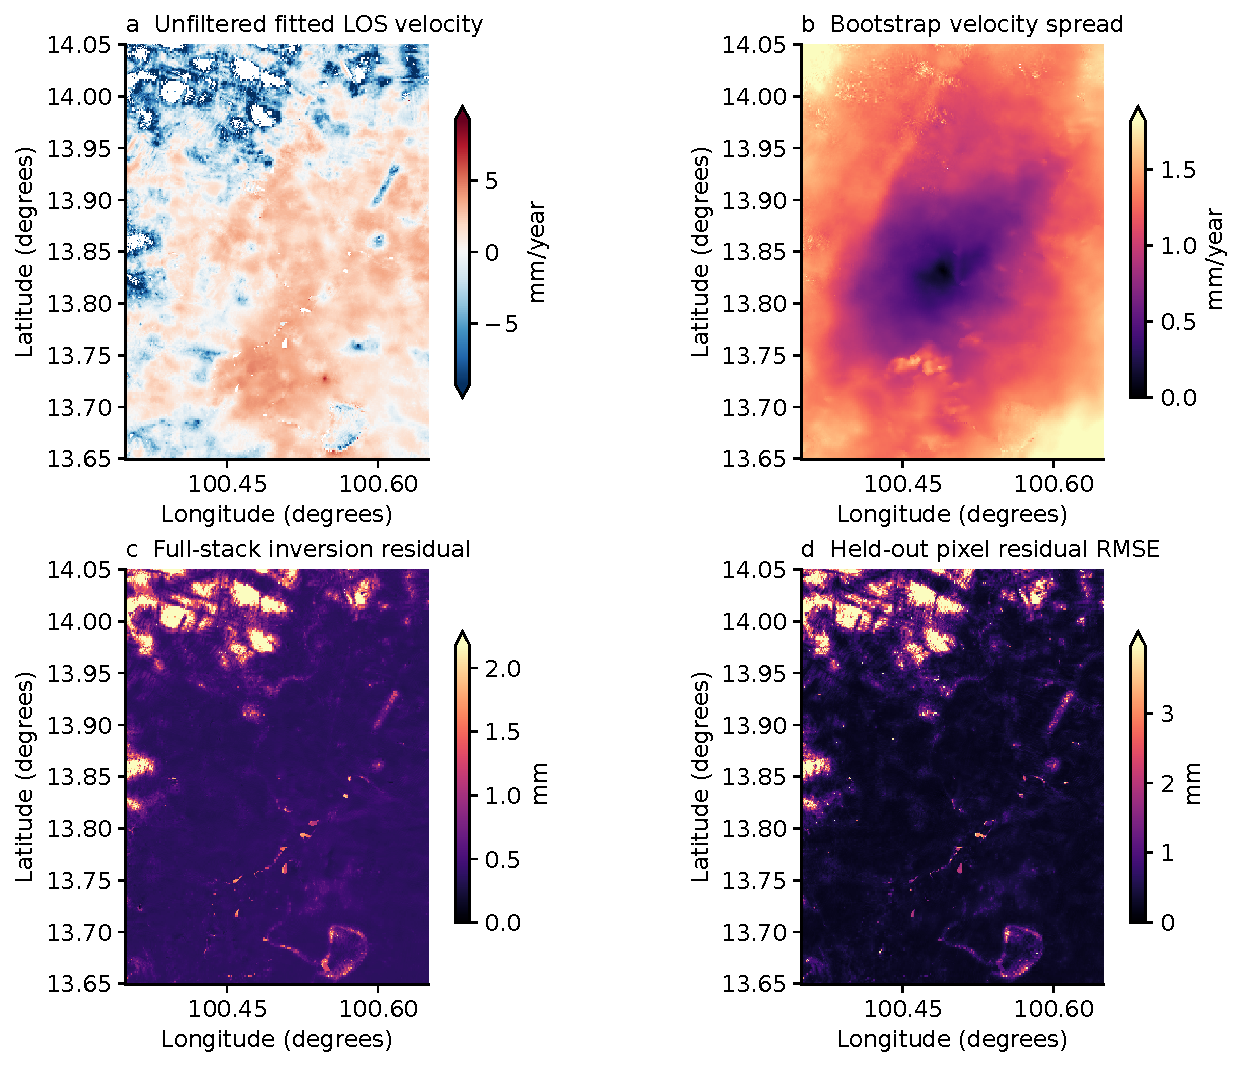
\includegraphics[width=\linewidth]{figures/S3_matched_quality.pdf}
\caption{Actual same-chain quality fields in the Bangkok processing rectangle. Panel a shows the unfiltered fitted LOS velocity only where the full quality mask passes. Other panels retain finite quality diagnostics and held-out RMSE. Symmetric velocity limits and the upper limits of other color scales use their 98th percentiles for readability; values outside those limits are clipped in color only and retained in the data. No map supplies independent GNSS accuracy or motion in unobserved locations.}\end{figure}


\clearpage
\section*{S8. Downstream exposure examples and the Iran provenance correction}
\footnotesize
\begin{longtable}{p{.24\linewidth}p{.38\linewidth}p{.3\linewidth}}
\caption{Targeted examples of downstream exposure practice and the scope supported by each study.}\\
\toprule Source & Reported measurement and population-transfer choices & Permitted interpretation for the present review\\\midrule\endfirsthead
\toprule Source & Reported measurement and population-transfer choices & Permitted interpretation for the present review\\\midrule\endhead
Blackwell et al. \citep{blackwell2020california} & California coastal VLM combines ALOS/Sentinel-1 and GNSS; community exposure is estimated assuming uniform population distribution within communities. & A community-scale transfer assumption materially defines the exposure estimate; the authors describe it as a guide for prioritizing detailed risk assessment, not a complete risk inventory.\\
Fern\'andez-Torres et al. \citep{fernandeztorres2024mexico} & Mexico-wide assessment applies a temporal-coherence threshold of 0.7, compares InSAR velocities with GPS, and estimates population/households in detected subsiding urban localities using census information. & The published exposure is tied to the mapped localities and screened observations; it does not by itself estimate deformation in areas without usable InSAR observations.\\
Ao et al. \citep{ao2024national} & Reports urban land and population shares above specified InSAR subsidence-rate thresholds across 82 major Chinese cities. & A population share associated with mapped urban subsidence classes; it should not be interpreted as a counterfactual estimate for unobserved city areas.\\
Ohenhen et al. \citep{ohenhen2025uscities} & 28 US cities mapped with WabInSAR at about 28-m resolution; rates were compared with 154 GNSS stations. Citywide summaries use area-weighted rates; 2020 census-block population is assigned to velocity classes using the median InSAR-pixel rate in each block. & A high-resolution, geodetically checked exposure workflow and a valuable alternative. Area-weighted city summaries and census-block median-rate assignments answer different questions from fine-grid population-weighted support; the paper is not evidence of downstream misuse.\\
Murray et al. \citep{murray2025hawaii} & Masks unreliable InSAR observations and combines retained VLM estimates with a lidar DEM for future coastal flood exposure. The discussion notes that subsidence between large buildings may remain undetected. & Explicitly recognizes a coverage limitation and calls for ground surveys or higher-resolution observations; this is evidence of responsible qualification, not misuse.\\
Aieorattanawadee \citep{aieorattanawadee2022bangkok} & Bangkok Sentinel-1 time series for 2018--2022 compared ascending and descending results with seven CORS stations; the thesis abstract reports agreement at four and two stations, respectively. & A local example of independent geodetic comparison, but sparse station coverage. The published abstract does not provide station-level series for reanalysis here, so it is not validation of our results.\\
Luachapichatikul \citep{luachapichatikul2020bangkok} & 2016--2019 descending Sentinel-1 PS versus leveling: leveling/PS relative rates (mm yr$^{-1}$) -3.32/-4.28, -7.08/-6.49, -2.62/-3.93 and -1.84/-0.88; PS-to-benchmark offsets 15.32, 196.59, 120.34 and 34.89 m; leveling-fit $R^2$ 0.82, 0.94, 0.86 and 0.10. & Three rate differences are 0.59--1.31 mm yr$^{-1}$, but PS is descending LOS while leveling is vertical; offsets are material, one fit is poor, and the sample is four selected pairs. This is validation practice context, not validation of our stack.\\
Pumpuang and Aobpaet \citep{pumpuang2024bangkapi} & Bang Kapi PS-InSAR compared with RTSD SBKK CORS over October 2019--February 2020; reports $r=0.88$ and RMSE 3.98 mm. InSAR at the station was unavailable, so the comparison used mean change within a 100-m buffer. & Directly relevant independent-validation practice, but one station and a buffered spatial target. The published summary is not raw validation data for our analysis.\\
Keerinart et al. \citep{keerinart2020sbkk} & A 23-week SBKK CORS analysis (2 October 2019--6 March 2020) reports a vertical ellipsoidal-height rate of 13.308 mm yr$^{-1}$; the authors note construction and pile driving at the station building during the observations. & A nearby-in-time geodetic record, but the authors identify a site disturbance that can make monument motion differ from regional ground motion. Its plotted samples are not machine-readable station data.\\
Haghshenas Haghighi and Motagh \citep{haghshenas2024iran} & Nationwide Sentinel-1 analysis of 2014--2020 observations; public annual-rate raster projected from LOS to vertical, a derived subsidence mask, and seasonal-amplitude raster. & The archived rate and mask are from this 2024 source, not a Motagh et al. (2008) nationwide rate product. These summaries do not provide the per-pair support field used in the primary experiment.\\
Payne et al. \citep{payne2025iran,payne2024data} & 2014--2022 analysis of 106 selected subsiding regions; ascending/descending data are decomposed into vertical and east--west velocities with 1-sigma uncertainties. Regions are screened by rate/area and interpretation criteria. & A newer and relevant scientific product, but its released component-velocity fields and selected-region masks are not pair-specific support masks. Its underlying LiCSAR interferograms are separately accessible; this study does not reprocess them for Iran because Iran is no longer a quantitative application domain.\\
LiCSBAS \citep{morishita2020licsbas} & Unwrapped-data checks, loop closure, inversion and multi-index quality masking. & Established processing quality; a sampled coherence diagnostic alone is insufficient.\\\bottomrule
\end{longtable}
\normalsize

\paragraph{Published local validation context.} Local validation practice is also relevant. A 2016--2019 Bangkok thesis compared descending Sentinel-1 PS rates with four deep leveling benchmarks. The reported vertical-leveling/descending-LOS relative-rate pairs were -3.32/-4.28, -7.08/-6.49, -2.62/-3.93 and -1.84/-0.88 mm yr$^{-1}$; the PS-to-benchmark offsets were 15.32, 196.59, 120.34 and 34.89 m, and the leveling-fit $R^2$ values were 0.82, 0.94, 0.86 and 0.10, respectively \citep{luachapichatikul2020bangkok}. The first three rate differences were 0.59--1.31 mm yr$^{-1}$, but the quantities are different motion components, the spatial offsets reach about 197 m, and only four pairs were reported. We treat this as evidence of local validation practice, not like-for-like validation of our products. A separate Bang Kapi study compared a five-month 2019--2020 InSAR time series with RTSD SBKK CORS, reporting $r=0.88$ and RMSE 3.98 mm, but used an average within 100 m because no InSAR observation was available at the station itself \citep{pumpuang2024bangkapi}. An earlier analysis of the same SBKK station used 23 weekly RINEX solutions from October 2019 to March 2020 and reported a vertical ellipsoidal-height rate of 13.308 mm yr$^{-1}$; its authors noted concurrent construction and pile driving at the station building, so the measured motion may include local site or structure effects \citep{keerinart2020sbkk}. A 2018--2022 Bangkok time-series thesis also compared ascending and descending results with seven CORS stations, reporting agreement at four and two stations, respectively \citep{aieorattanawadee2022bangkok}. These examples establish that independent geodetic checks are used in the region, while their small station counts, spatial offsets, site conditions or interval-specific targets limit transfer to our study. The published abstracts and summaries do not provide complete machine-readable, time-tagged station observations and processing metadata needed for our own matched reanalysis. 

\paragraph{SBKK support check in the separate LiCSAR stack.} The published RTSD coordinate for SBKK (13.792944$^\circ$ N, 100.596494$^\circ$ E) lies inside the matched LiCSAR subregion \citep{jica2024thailandcors}. At this coordinate, the nearest LiCSAR grid-cell center is 44.8 m away and passes the final LiCSBAS mask. Two pixel centers lie within a 100-m radius, and both pass the mask; their median velocity is 2.314 mm yr$^{-1}$ in LOS. This is a product-specific support audit, not GNSS validation. It differs from the cited PS-InSAR study because the sensor product and processing chain differ. We do not compare the LOS rate directly with the published SBKK ellipsoidal-height rate: the motion components and reference frames differ, and the SBKK paper reports construction and pile driving during the GNSS interval. The acquisition-level series and calculation are retained in \path{results/gnss_feasibility/SBKK_100m_LiCSAR.csv}, \path{results/gnss_feasibility/SBKK_support_summary.json} and \path{audit_sbkk_support.py}.

The archived Iran rate and mask match the official Zenodo 10815578 files by MD5 (respectively \path{c0a19300c161940dc2e6a8de267cef4f} and \path{734c58f4f2f2fbc7017d705f9b81fe3d}). This establishes the archive provenance only; neither raster enters an exposure result. The archived seasonal-amplitude file does not match that release and is also unused. Although Payne et al. make regional time-series velocities available through the COMET-LiCS Subsidence Portal and the source interferograms through the LiCSAR portal, those materials were not ingested into this Iran-free primary experiment. Thus there is no claim that a suitable newer dataset is inaccessible or inferior; the correction is that the supposed 2008 Iran application was a misattributed, exploratory parser branch, not a justified choice of scientific dataset. The file-level audit is retained in \path{results/lineage/iran_actual_file_match.json}.

The evidence examples were selected for direct relevance, not through a systematic search designed to estimate prevalence. They document that population exposure is reported at different spatial units and that some studies explicitly discuss support limitations. They do not demonstrate widespread downstream misuse, nor does silence about a denominator prove that an author omitted quality control. The Iran parser demonstration is not restored as an independently validated exposure comparison. Older EGMS point-based sums are also not restored: counting an entire population pixel once for every point violates the required nonduplicated area accounting, and an LOS component cannot be relabeled vertical without a geometric decomposition.

\section*{S9. Reproduction and result-to-claim mapping}
The experiment directory separates source manifests, configuration, computed results, figures and manuscript sources. \texttt{paper/number\_ledger.json} records generated numerical macros and their source CSVs. The numerical checks verify geometry and accounting; the real-data comparisons and controlled masking address scientific sensitivity under their stated assumptions. No result validates unobserved subsidence simply because an implementation check passes.

\begin{tabular}{p{.22\linewidth}p{.69\linewidth}}\toprule
Claim/evidence & Authoritative result location\\\midrule
Historical reproducibility & \texttt{results/lineage/archive\_branches.csv}; factorial center-rule audit\\
Native support summaries & \texttt{results/fine/allocation\_summary.csv}, \texttt{support\_curves.csv}\\
Scale and origin effects & \texttt{results/allocation/scale\_origin\_comparison.csv}\\
Controlled failures and bounds & \texttt{results/masking/replicates.csv}, \texttt{synthetic\_hazard\_bounds.csv}\\
Sampling dependence & \texttt{results/sampling/}; date network and retained rank plans\\
Population and cover sensitivity & \texttt{results/population/}; own and common coverage reported\\
Second-region geometry & \texttt{results/dwr/}; actual polygon-union audit and repeat masking\\
Matched processing & \texttt{results/timeseries/}; stage logs, configuration and holdout records\\
Published benchmark context & \texttt{results/literature/bangkok\_leveling\_pairs.csv} and source audit JSON; source thesis linked in the bibliography.\\\bottomrule
\end{tabular}
\begin{figure}[htbp]\centering
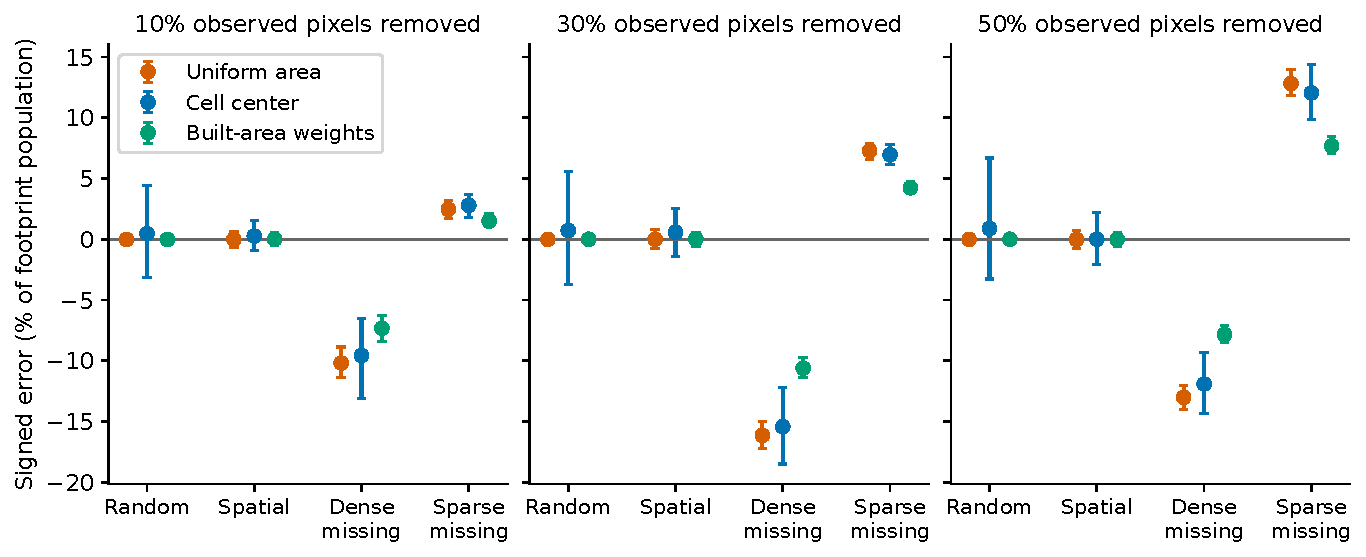
\includegraphics[width=\linewidth]{figures/S4_dwr_masking.pdf}
\caption{Controlled masking within the original Fresno observation footprint. ``Dense'' and ``sparse'' indicate preferential removal from higher- and lower-density fine locations. Identical masks are supplied to all three methods. Symbols and bars summarize 100 repetitions by their means and central 95\% mask ranges, conditional on the fixed GHSL reference. The denominator is population originally allocated inside the published footprint; the figure does not evaluate motion outside that footprint.}\end{figure}

\section*{S10. Method choices and comparison scope}
\begin{longtable}{p{.19\linewidth}p{.34\linewidth}p{.38\linewidth}}
\caption{Relationship to existing methods and the evidence supplied by this study.}\\
\toprule Approach & Required information and interpretation & Evaluation here\\\midrule\endfirsthead
\toprule Approach & Required information and interpretation & Evaluation here\\\midrule\endhead
Center sampling & Coarse population totals and support at a representative center; subcell support is assumed representative. & Same-input scale/origin comparisons; boundary effects separated; controlled-mask variability retained.\\
Uniform areal allocation & Coarse totals and support-area fractions; population assumed uniform over included area \citep{eicher2001dasymetric}. & Main method contrast, local errors, covariance decomposition, opposite-direction and small-bias scenarios.\\
Native-model allocation & Fine population model and intersected support; uniformity remains within each source population pixel. & Controlled reference with conserved first and cross moments; retains model detail without household validation.\\
Built-area weighting & Coarse totals and fine ancillary building surface, consistent with dasymetric allocation principles \citep{mennis2003population}. & Tested under introduced masks; shared information with GHSL limits independence.\\
Observed-domain overlay & Population assigned only to a stated valid observation footprint. & Fresno uses actual DWR cell polygons and their nonduplicated union; no inferred motion in gaps.\\
Processing quality diagnostics & Interferogram network, inversion outputs and multiple quality criteria \citep{morishita2020licsbas,yunjun2019mintpy}. & Full/train LiCSBAS branches and excluded-edge residuals; not equated with the primary sampled-support statistic.\\
Imputation or additional sensors & An explicit deformation model or additional independent observations with compatible references. & Discussed as information needed for missing deformation; no numerical superiority over these different-target methods is claimed.\\\bottomrule
\end{longtable}

Uniform allocation is adequate for the chosen model target when within-cell population--support covariance is negligible at the required reporting scale. Native allocation retains that covariance when fine input information is available. These are conditional choices; a method that retains inaccurate fine population structure is not thereby demographically validated. Complete-case summaries remain valid for their explicitly observed domain. The contribution here is the matched-input evaluation and quantified applicability, rather than the invention of areal interpolation or an accounting identity.

\section*{S11. Boundary sensitivity and internal computational recheck}
For the primary $q=0.3$ population field, an additional implementation constructs the geographic domain from the union of native GHSL mask pixels. Edges are densified at native-pixel spacing before transformation to UTM. Coarse squares fully covered by this boundary form the complete-interior subset; all remaining included squares form the partial-boundary subset. Different origins produce different interior subsets, so each row uses its own population and reference deficit. The main full-domain estimator is unchanged. The metric moments were freshly reprojected and reaggregated with independently constructed interval weights; all 32 primary method/scale/origin estimates agree with the retained table within $10^{-4}$ population units.

\begin{table}[htbp]\centering\small
\caption{One-kilometre uniform allocation after excluding boundary-crossing squares. Deficits are in million mean population-allocation units. Relative difference uses the interior reference; population share uses the original whole-domain total.}
\begin{tabular}{rrrrrr}\toprule
Origin shift (m) & Cells & Pop. share (\%) & Native & Uniform & Difference (\%)\\\midrule
(0, 0) & 14,120 & 99.49 & 2.960 & 4.685 & 58.29\\
(500, 0) & 14,107 & 99.39 & 2.950 & 4.668 & 58.24\\
(0, 500) & 14,123 & 99.41 & 2.955 & 4.685 & 58.56\\
(500, 500) & 14,111 & 99.27 & 2.944 & 4.664 & 58.46\\
\bottomrule\end{tabular}

\end{table}

The interior contrast remains \InteriorBiasMin{}--\InteriorBiasMax{}\%, compared with \UniformBiasMin{}--\UniformBiasMax{}\% across the full domain. The separate center-outside subset quantifies the explicitly declared zero-support boundary rule in the center method. Full per-origin tables retain cell counts, denominators, signed errors, absolute cell-error sums and positive/negative cell counts for both methods. Files are in \path{revision_round2/evidence/boundary_allocation.csv}.

For native support, a separate nested-rectangle intersection calculation checked 80 deterministic random/support-extreme pixels for every original pair and all four support definitions (8,960 comparisons). The largest support-fraction difference was $2.98\times10^{-8}$, consistent with float32 storage. Actual GeoTIFF tiepoints, pixel scales and point registration were independently compared with GDAL transforms for both raster types. These are sampled spatial checks, not exhaustive independent reprocessing of every native pixel.

The internal recheck reconstructed all 44 held-out edge residuals directly from retained phases and the training HDF5 series, verified 393 training memberships, and recalculated the training-only support bins. The largest difference in grouped RMSE was $7.27\times10^{-7}$ mm under independent float64 arithmetic, compared with reported precision of 0.001 mm. Each evaluable pixel--edge observation receives equal weight; none of these counts is assumed to be an independent physical replicate.

Each region's complete 21,600-row controlled-mask factorial was checked for coverage and arithmetic. Repetitions 0, 1, 49 and 99 were regenerated for all mechanisms and removal fractions at the 10-pixel zero-origin setting, independently recalculating 144 method results per region. All 400 conditional sampling draws and all 64 population-model/coverage/support summary rows were recalculated. Nested mean fields are stored as float32, so averaging already-integrated pair totals and integrating a stored mean can differ slightly; the maximum observed difference was $1.35\times10^{-8}$ of the corresponding total exposure.

For Fresno, an independent global union of the original polygon rings differs from the stored covered-area sum by 0.0019 m$^2$ over approximately 388.9 km$^2$; 128 deterministic random pixel intersections agree within $2.34\times10^{-11}$ in support fraction. All 1,260 distinct original radar rasters referenced by the legacy, expanded and matched manifests match their recorded checksums after relocation. The manifests retain their original paths as provenance; an explicit resolver rebases known roots and rejects missing or ambiguous inputs. These are internal implementation checks with defined scope; they do not provide independent physical or demographic validation.


\clearpage\section*{S12. Crossed population-model and pair-selection sensitivity}
The common domain contains 1,754,190 native GHSL pixels and 22,357,666.843 GHSL population units; 142,949.221 GHSL units from the full primary footprint are excluded. It intersects the primary footprint with full coverage of GHSL 2020 and WorldPop 2020 only; the four-layer epoch comparison in S6 uses a separately defined intersection. Each model is normalized to the GHSL total in this two-model domain before any support calculation. We cross these two allocations with the original 28-pair and expanded 224-pair mean joint support fields, at $q=0.3$. Neither population product is treated as demographic truth.

All comparisons use 1-km cells in UTM zone 47N and offsets $(0,0)$, $(500,0)$, $(0,500)$ and $(500,500)$ m. Within each combination, native-model and uniform allocations have identical cell population totals and the same included-domain area. We project extensive area, supported area, population and supported population separately onto a 50-m integration grid. The population--support product is formed before projection. Retaining partial cells avoids full-cell extrapolation outside the domain.

\begin{table}[htbp]\centering\footnotesize
\caption{Crossed population-model and pair-selection comparison at 1 km and $q=0.3$. Both models use the same domain and total. Deficits and differences are in millions of allocation units (M). Ranges span four grid origins; they are not confidence intervals. $\Delta=U_{\rm uniform}-U_{\rm native}$, and pp denotes percentage points of the common total.}\label{tab:cross}
\setlength{\tabcolsep}{3.5pt}
\begin{tabular}{llrrrrr}\toprule
Model & Pairs & Native (M) & Uniform (M) & $\Delta$ (M) & $\Delta$/native (\%) & $\Delta$/total (pp)\\\midrule
GHSL & 28 & 2.989 & 4.645--4.653 & 1.656--1.663 & 55.38--55.64 & 7.40--7.44\\
GHSL & 224 & 3.268 & 4.944--4.951 & 1.676--1.683 & 51.29--51.51 & 7.50--7.53\\
WorldPop & 28 & 5.186 & 5.654--5.657 & 0.468--0.471 & 9.03--9.07 & 2.09--2.10\\
WorldPop & 224 & 5.488 & 5.963--5.965 & 0.474--0.476 & 8.64--8.68 & 2.12--2.13\\
\bottomrule\end{tabular}\end{table}

Production first and cross moments conserve source totals to relative tolerance $10^{-8}$, and aggregation over each origin preserves those projected totals. Direct native-grid integration agrees with the coarse cross-moment reference. The 25-m diagnostic retains raw reprojection drift without renormalization (maximum absolute relative moment drift 1.65e-05). Its maximum change in uniform-minus-native difference is 0.000436 percentage points of the common total, below the prespecified 0.01-percentage-point numerical tolerance. These are numerical sensitivity checks, not uncertainty intervals.

All 16 production rows have positive uniform-minus-native differences. GHSL gives a larger effect than WorldPop under both pair selections. The result supports a persistent direction for these selected inputs, while showing that a single percentage cannot represent population-model sensitivity. Because pair number and pair composition change together, no causal effect of sample size is inferred. The four origins are deterministic sensitivity cases, not independent replicates.

\begin{figure}[htbp]\centering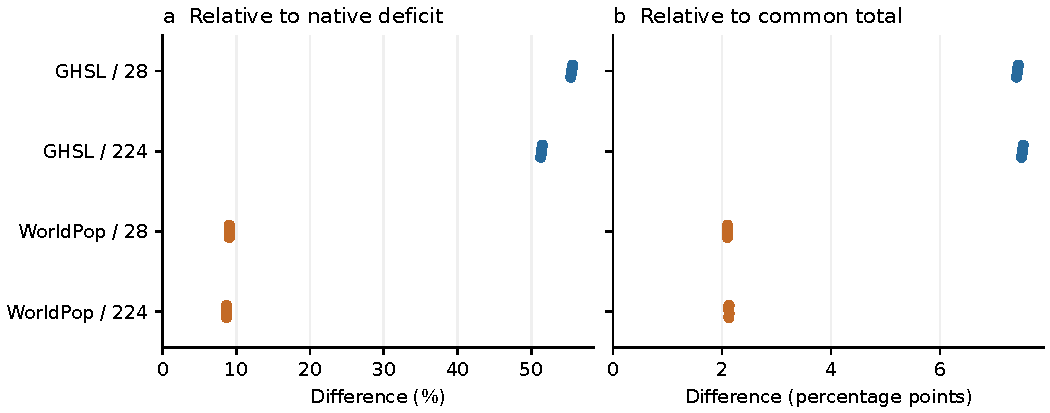
\includegraphics[width=\linewidth]{figures/S5_cross_sensitivity.pdf}
\caption{Crossed aggregation sensitivity. Dots show four grid origins and horizontal lines span them. Left: difference relative to the native-model deficit. Right: the same difference as percentage points of the common population total. Colors identify population model; the 28 and 224 labels identify distinct pair selections.}\label{fig:cross}
\end{figure}

Complete 16-row results, the 25-m comparison, conservation ledger and input SHA-256 values are retained in \path{results/cross_sensitivity/}. The analysis and figure can be regenerated with \path{experiment_cross_sensitivity.py} and \path{make_cross_sensitivity_paper.py}.

\clearpage\section*{S13. Paired input-support and final-quality-mask allocation}
We compared two separate support quantities on the same 401-by-301 LiCSBAS grid and the same fixed GHSL population field: (i) the mean coherence-and-unwrapped support across all 437 input pairs, and (ii) the final full-stack LiCSBAS quality mask. The first is a per-pixel input-pair support fraction; the second is a binary product-level quality decision. They are not interchangeable measurements. For each field we retained population, spherical pixel area, area-times-support and population-times-support separately. We compared native-cell deficits with uniform redistribution within 1-km UTM cells at four zero/half-cell origins.

The direct-geometry audit independently intersected each coarse UTM cell with the original 0.001-degree source cells in longitude-radians/sine-latitude equal-area coordinates. Inverse-projected cell boundaries were densified at 24 segments per edge. This is independent of GDAL raster reprojection and preserves partial edge cells. Uniform-within-source-pixel population and support are assumed during the subpixel intersection. Across all four origins, population mass drift was below $2\times10^{-9}$ allocation units and spherical-area drift was below $10^{-6}$ m$^2$ at printed precision. The direct integration agrees with the refined 25-m raster calculation to the reported 0.01-percentage-point gate.

\begin{table}[htbp]\centering\scriptsize
\caption{One-kilometre allocation effects from direct source-cell intersections. Differences are signed percentage points of the fixed AOI population; positive values indicate a larger deficit under uniform-area allocation than under native population allocation.}
\begin{tabular}{p{2.5cm}p{2.2cm}p{3.8cm}p{4.0cm}}\toprule
Support definition & Native deficit (\% population) & Uniform-area effect (pp; four origins) & Interpretation\\\midrule
437-pair mean input support & 3.4539 & +3.0662 to +3.1891 & Input-pair support frequency\\
Final full-stack quality mask & 0.2944 & +0.1077 to +0.1170 & Product-level accepted/rejected mask\\\bottomrule
\end{tabular}
\end{table}

Both definitions retain an allocation effect after coarse aggregation, but the magnitude differs by more than an order of magnitude. This difference is expected because a 437-pair mean support fraction and a final multi-index mask encode different processing information. It is not an error comparison between them, and neither establishes deformation or resident counts in invalid locations. All origin-specific cell intersections and checksums are retained in \path{direct_geometry_audit/} and \path{paired_support_pilot/}.

\clearpage\section*{S14. Artificial masking of observed LOS classes}
We used the unfiltered fitted LOS velocity from the full LiCSBAS branch, positive toward the satellite, only inside the final full-stack validity mask. The observed-domain reference contains 117,103 of 120,701 grid cells and 11.281 million GHSL allocation units. Population-weighted shares at or below $-2$, $-5$ and $-10$ mm yr$^{-1}$ are 2.474\%, 0.2805\% and 0.0223\%, respectively. These are relative LOS classes and are not vertical-settlement or hazard thresholds.

For each of 100 seeded repetitions, we artificially removed 10\% or 30\% of otherwise valid cells under four mechanisms: random, spatially clustered, preferentially high velocity spread, and preferentially low velocity spread. The latter two scores include a small seeded spatial perturbation so that replicates vary while remaining associated with the quality diagnostic. We estimated the threshold-class population among artificially masked cells from the within-block observed-population prevalence and from the nearest observed pixel to each block center. Nominal cell sizes were 5, 10 and 20 source pixels (about 0.55, 1.11 and 2.22 km); four zero/half-cell origins retain partial raster-edge blocks. The known hidden class population is calculated directly from the observed LOS values before artificial masking. Every comparison therefore has a defined conditional reference.

\begin{table}[htbp]\centering\scriptsize
\caption{Observed LOS population-class masking, 30\% removed cells, nominal 1.11-km blocks, threshold $v_{LOS}\leq-5$ mm yr$^{-1}$. Estimates and biases are GHSL model allocation units, not verified person counts. Bias ranges are the 2.5th--97.5th percentiles across seeded masks and the four grid origins; they are design-sensitivity ranges, not confidence intervals.}
\begin{tabular}{llrrrr}\toprule
Removal pattern & Estimator & Known hidden class & Mean bias & Relative bias (\%) & Bias range\\\midrule
Random & Local observed prevalence & 9,514 & 91 & 1 & $[-835,1194]$\\
Random & Nearest observed centre pixel & 9,514 & 9,455 & 100 & $[6,139,13,265]$\\
Spatial clusters & Local observed prevalence & 9,542 & 153 & 5 & $[-5,596,7,924]$\\
Spatial clusters & Nearest observed centre pixel & 9,542 & 4,368 & 52 & $[-2,803,15,074]$\\
High-spread selection & Local observed prevalence & 16,657 & $-5,018$ & $-30$ & $[-9,879,1,332]$\\
High-spread selection & Nearest observed centre pixel & 16,657 & $-1,952$ & $-12$ & $[-8,068,6,793]$\\
Low-spread selection & Local observed prevalence & 1,375 & 1,079 & 79 & $[-453,3,357]$\\
Low-spread selection & Nearest observed centre pixel & 1,375 & 1,566 & 114 & $[-77,4,924]$\\\bottomrule
\end{tabular}
\end{table}

The local prevalence estimator is close to aggregate reference under random masking, while center sampling overestimates the $-5$ mm yr$^{-1}$ class in that case. Under quality-selective removal the local estimator has a negative or positive bias depending on which velocity-spread tail is removed; spatial clustering also broadens the conditional range. Velocity spread is a processing diagnostic, not a calibrated uncertainty interval. Across all three predeclared LOS thresholds and all scales, neither estimator is uniformly accurate across mechanisms. The complete factorial is retained in \path{actual_los_masking/replicates.csv}, with grouped summaries in \path{actual_los_masking/summary.csv}.

This experiment is closer to the observed product than synthetic two-valued fields, but remains conditional on a fixed population model, the final valid domain and known observed velocities. Original invalid pixels are excluded before artificial masking. It does not validate motion or exposure in permanently unobserved locations.


\clearpage
\section*{S15. Covariance identity and scale sensitivity diagnostic}

For a reporting square containing fine pixels $i$, let $A_i$ be pixel area, $s_i\in[0,1]$ the observed-support fraction and $\rho_i=p_i/A_i$ the native population density. With the same total population and geographic square held fixed, the difference between the area-uniform and native-population support deficits is
\begin{equation}
D_{\mathrm{uniform}}-D_{\mathrm{native}}
=\frac{\operatorname{Cov}_{A}(\rho,s)}{\bar{\rho}_{A}},
\end{equation}
where area-weighted moments are calculated over the square and $\bar{\rho}_{A}=\sum_i A_i\rho_i/\sum_i A_i$. The absolute difference is bounded by $\sigma_{\rho,A}\sigma_{s,A}/\bar{\rho}_{A}$ by Cauchy--Schwarz. This identity describes the accounting mechanism; it is not an empirical uncertainty interval.

We checked this identity on a fixed common domain of 120,175 pixels, crossing the GHSL and common-total-normalized WorldPop surfaces with the 437-pair mean input-support field and the final full-stack quality mask. Projected pixel centres were assigned to 250-, 500-, 1,000- and 2,000-m squares at four grid origins. The resulting scale/origin ranges are:

\begin{table}[htbp]\centering\small
\caption{Uniform-minus-native deficit and Cauchy--Schwarz upper bound across projected square sizes and grid origins. Values are percentage points. Pixel-centre grouping is a sensitivity diagnostic and differs from the direct polygon-intersection integration used for the primary 1-km result.}
\begin{tabular}{llrr}\toprule
Support field & Population surface & Difference range & Bound range \\
\midrule
437-pair mean & GHSL & 0.550--4.670 & 1.076--9.599 \\
437-pair mean & WorldPop, normalized & 0.164--2.376 & 0.429--5.320 \\
Final quality mask & GHSL & 0.012--0.241 & 0.088--1.967 \\
Final quality mask & WorldPop, normalized & 0.010--0.197 & 0.054--1.200 \\
\bottomrule\end{tabular}
\end{table}

The covariance identity residual is at most $1.22\times10^{-15}$ percentage points across all 64 model--support--scale--origin combinations, and no observed absolute difference exceeds its corresponding bound. These numerical checks confirm implementation consistency only. The grouped-square differences are not pooled with the primary exact-geometry estimate; their spread across scales and origins is design sensitivity, not a confidence interval. WorldPop is a model-sensitivity comparison, not independent demographic truth, and the two products may share census inputs. Input checksums, full scenario definitions, local effects and machine-readable results are retained with the analysis outputs.

\clearpage
\section*{S16. Fresno 2020 Census-block support overlay}

We intersected 2020 Census demographic and housing characteristics block polygons and total-population counts (field P0010001) with the fixed Fresno region of interest used in the DWR analysis. The block service identifies the U.S. Census Bureau DHC tables and TIGER geodatabase as its sources, reports the 2020 vintage, and notes differential-privacy protection of Census counts. We queried 6,999 unique Fresno County block GEOIDs intersecting the ROI; 6,788 complete blocks lie wholly inside its boundary and contain 523,953 Census population, 96.44\% of the population in all intersecting queried blocks. The complete-block restriction avoids assigning an entire block population to a partial ROI intersection.

The DWR layer supplies 38,738 published observation polygons, not velocity estimates. We rasterized complete block polygons and the DWR polygon union at fivefold and tenfold supersampling of the 3-arc-second GHSL grid and weighted subpixels by spherical area. For each complete block, the area-uniform Census estimator assigns its population count in proportion to the fraction of block area inside the union of DWR observation polygons. The block-median-observability estimator classifies a block as observed when at least half of its area is covered, then assigns the whole block population to that category. A separate 90\% area-coverage threshold is reported as a sensitivity. These are block-level support statistics, not median-velocity classes.

\begin{table}[htbp]\centering\small
\caption{Fresno Census-block support estimates. All rates refer to published observation-footprint coverage, not deformation velocity. The complete-block population is 523,953 in both rasterization runs.}
\begin{tabular}{lrr}\toprule
Quantity & 5$\times$ & 10$\times$ \\
\midrule
DWR-observed area within rasterized complete blocks (km$^2$) & 366.903 & 366.892 \\
Share of complete-block land area covered by DWR polygons (\%) & 79.761 & 79.764 \\
Census population-weighted support, uniform within block (\%) & 99.186 & 99.192 \\
Census population in blocks with $\geq$50\% observed area (\%) & 99.406 & 99.410 \\
Census population in blocks with $\geq$90\% observed area (\%) & 98.076 & 98.034 \\
Native GHSL population-weighted support on the same block domain (\%) & 99.739 & 99.739 \\
GHSL minus Census-uniform support share (percentage points) & 0.553 & 0.547 \\
\bottomrule\end{tabular}
\end{table}

At tenfold resolution, 6,784 of 6,788 blocks receive rasterized area; the four blocks without rasterized subpixels have zero Census population. The median ratio of rasterized block area to Census ALAND+AWATER is 0.9999. The fivefold-to-tenfold change is at most 0.042 percentage points across the reported support shares. The native GHSL allocation total in these same complete blocks is 587,868, 12.20\% above the 523,953 Census count. Accordingly, the 0.55-point support-share contrast combines differences in population totals and spatial allocation; it is not a calibrated error estimate or independent population validation.

This support overlay by itself does not reproduce published Census-block median-rate classification: the DWR polygon layer contains no velocities. We therefore added a separate DWR/TRE ALTAMIRA vertical-rate raster analysis in S17. Census and GHSL counts may share source inputs; the Census counts are differentially private. The DWR observation polygons span 2015--2026 whereas the population epoch is 2020. Neither analysis imputes deformation outside the footprint or validates hazard exposure. The service responses, rasterization script, per-block tables, grid-resolution checks and SHA-256 values are retained in the analysis bundle.

\clearpage
\section*{S17. Census-block median vertical-rate classification in Fresno}

To compare with published block-median exposure workflows, we obtained raw floating-point annual-rate and cumulative vertical-displacement rasters from the California DWR TRE ALTAMIRA ImageServer. DWR documents the annual layers as Sentinel-1-derived vertical displacement rates, with an approximately 100-m pixel size and values in feet per year; the public raster products are interpolated from point measurements \citep{dwr2026,dwrdocumentation}. The six annual rate layers from October 2015--October 2016 through October 2020--October 2021 were exported at their native EPSG:4326 grid size with nearest-neighbour sampling and aspect-ratio adjustment disabled. We built a pixelwise temporal median, retaining only cells valid in all six layers. The temporal-median vertical rate at each DWR cell was then sampled within the published 100-m observation-cell polygons and assigned to Census blocks by polygon membership. The 38,738 observation polygons map exactly to 38,738 native-grid cells in the snapped export. Census-block population is assigned to the median rate within each block, following the transfer step used by Ohenhen et al. \citep{ohenhen2025uscities}. Rates were converted from feet per year to millimetres per year by multiplying by 304.8.

For the six-window temporal median, 6,129 complete Census blocks have valid cells and contain 501,411 people, 95.70\% of the 523,953 residents in all 6,788 complete blocks. Blocks with no valid cell are left unclassified rather than assigned to a rate class. The thresholds are VLM $\geq 0$, $-3\leq$ VLM $<0$, $-5\leq$ VLM $<-3$, $-10\leq$ VLM $<-5$, and VLM $<-10$ mm yr$^{-1}$, matching the categories in the published comparator. Table~S14 reports class-specific populations for the temporal-median and endpoint-rate estimates; Table~S15 summarizes annual-rate sensitivity.

\begin{table}[htbp]\centering\small
\caption{Fresno 2020 Census population assigned to DWR vertical-rate classes using the median rate in each block. The temporal median uses six October-to-October windows in 2015--2021; the endpoint rate annualizes cumulative displacement from June 2015 to January 2021. Each covers blocks containing 501,411 people.}
\begin{tabular}{p{.28\linewidth}p{.38\linewidth}rr}\toprule
Temporal estimator & Median-rate class (mm yr$^{-1}$) & Population & Share (\%) \\\midrule
2015--2021 temporal median & VLM $\geq0$ & 0 & 0.00 \\
2015--2021 temporal median & $-3\leq$ VLM $<0$ & 42 & 0.01 \\
2015--2021 temporal median & $-5\leq$ VLM $<-3$ & 174,288 & 34.76 \\
2015--2021 temporal median & $-10\leq$ VLM $<-5$ & 312,467 & 62.32 \\
2015--2021 temporal median & VLM $<-10$ & 14,614 & 2.91 \\
Endpoint rate & VLM $\geq0$ & 0 & 0.00 \\
Endpoint rate & $-3\leq$ VLM $<0$ & 197,045 & 39.30 \\
Endpoint rate & $-5\leq$ VLM $<-3$ & 208,738 & 41.63 \\
Endpoint rate & $-10\leq$ VLM $<-5$ & 90,844 & 18.12 \\
Endpoint rate & VLM $<-10$ & 4,784 & 0.95 \\
\bottomrule\end{tabular}
\end{table}

\begin{table}[htbp]\centering\small
\caption{Annual-rate temporal sensitivity. Population percentages refer to Census residents in rate-covered blocks and are assigned by the median annual rate in each block.}
\begin{tabular}{lrrrr}\toprule
Annual window & Median DWR rate (mm yr$^{-1}$) & Coverage (\%) & VLM $<0$ (\%) & VLM $<-5$ (\%) \\\midrule
2015--2016 & $-6.05$ & 95.70 & 100.00 & 70.05 \\
2020--2021 & 7.27 & 95.70 & 0.81 & 0.17 \\
2023--2024 & $-2.67$ & 95.70 & 92.18 & 22.94 \\
2025--2026 & $-9.18$ & 95.70 & 100.00 & 99.86 \\
\bottomrule\end{tabular}
\end{table}

For the 2015--2021 temporal-median surface, 65.23\% of the rate-covered population falls in blocks with median vertical rates below $-5$ mm yr$^{-1}$. Allocating each block population uniformly among its valid DWR cells instead of assigning all residents to the within-block median changes any class share by at most 0.15 percentage points in this period. The annual snapshots vary markedly; for example, the median rate among DWR cells changes from $+7.27$ mm yr$^{-1}$ in 2020--2021 to $-9.18$ mm yr$^{-1}$ in 2025--2026. The cumulative endpoint mean rate from June 2015 to January 2021 also gives a different block-class distribution from the six-window temporal median. This illustrates temporal-estimand sensitivity and cautions against treating one annual product as a multi-year trend.

To make temporal sensitivity explicit at the block level, we cross-tabulated the median-rate class from the 2015--2021 six-window surface against the 2025--2026 single-year surface using only the same 6,129 blocks with valid rates in both products. We hold the 2020 Census population fixed in both columns to isolate reclassification; the later column is therefore not a contemporaneous 2025--2026 exposure estimate. Of the 501,411 residents in these common blocks, the share assigned to rates below $-5$ mm yr$^{-1}$ rises from 65.23\% to 99.87\%, and 60.88\% of residents change at least one class. This is a temporal-product sensitivity, not evidence that long-term hazard changed by that amount: the comparison is between a six-year median and one annual estimate. Table~S16 reports the full population transition matrix.

\begin{table}[htbp]\centering\small
\caption{Fixed 2020 Census population (people) cross-classified by each block's median DWR vertical rate in 2015--2021 and 2025--2026. Only the 6,129 blocks with valid observations in both periods are included (501,411 residents). The 2025--2026 values are a single-year sensitivity, not a long-term rate or contemporaneous population exposure.}
\begin{tabular}{lrrrrr}\toprule
\shortstack{2015--2021 class\\(mm yr$^{-1}$)} & \multicolumn{5}{c}{2025--2026 class (mm yr$^{-1}$)} \\
 & $\geq0$ & $[-3,0)$ & $[-5,-3)$ & $[-10,-5)$ & $<-10$ \\
\midrule
$\geq0$ & 0 & 0 & 0 & 0 & 0 \\
$[-3,0)$ & 0 & 0 & 0 & 42 & 0 \\
$[-5,-3)$ & 0 & 0 & 668 & 172,826 & 794 \\
$[-10,-5)$ & 0 & 0 & 0 & 180,893 & 131,574 \\
$<-10$ & 0 & 0 & 0 & 0 & 14,614 \\
\bottomrule\end{tabular}
\end{table}

We further tested persistence across the six consecutive October-to-October annual products used in the 2015--2021 temporal median. For each year, we first calculated the median valid vertical rate within each Census block; we then counted how many of the six yearly block medians were below $-5$ mm yr$^{-1}$. Among the same 6,129 blocks with valid rates in every window (501,411 residents using fixed 2020 counts), 95.06\% of residents are in blocks that cross this threshold in one to five windows, and 0.10\% are in blocks below the threshold in all six. Thus 95.16\% cross the threshold in at least one window, while 4.84\% are never below it. This confirms that single-window classifications are temporally variable in the DWR product; it does not establish which annual rate is correct or imply persistent long-term hazard. Table~S17 gives the population distribution by number of years below the threshold.

\begin{table}[htbp]\centering\small
\caption{Persistence of the block-median $-5$ mm yr$^{-1}$ threshold across six consecutive annual DWR products from October 2015 to October 2021. Population uses fixed 2020 Census counts. The denominator is the 6,129 complete blocks with valid DWR cells in every annual window (501,411 residents).}
\begin{tabular}{rrrr}\toprule
Years below $-5$ & Blocks & 2020 Census population & Common population (\%) \\\midrule
0 & 364 & 24,268 & 4.84 \\
1 & 521 & 36,867 & 7.35 \\
2 & 864 & 60,973 & 12.16 \\
3 & 1,337 & 114,969 & 22.93 \\
4 & 1,874 & 167,416 & 33.39 \\
5 & 1,155 & 96,441 & 19.23 \\
6 & 14 & 477 & 0.10 \\\bottomrule
\end{tabular}
\end{table}

This transfer test uses an interpolated DWR/TRE ALTAMIRA vertical-rate raster, not our original LOS velocities, and shares provider lineage with the footprint product. It is not independent InSAR validation and cannot validate motion beyond the measured footprint; DWR vintage differences and Census differential privacy also limit interpretation. Scripts, cropped rasters, per-block data and checksums are in the analysis bundle.

\clearpage
\section*{S18. Spatial decomposition of Bangkok support-allocation effects}

To show whether the AOI-wide allocation effect hides local reversals or changes in low-support labels, we grouped the matched Bangkok processing grid into projected 1-km and 5-km squares aligned to integer-kilometre coordinates in UTM Zone 47N. Within each square, the native estimate weights the pixel support by the GHSL allocation; the area-uniform estimate applies the square's area-weighted support fraction to the same square population total. The reported difference is uniform minus native missing-support population, divided by the fixed AOI allocation total. Pixel-centre grouping is used here as a local diagnostic and is kept separate from the source-cell-intersection primary estimates.

At 1 km, the difference is 3.194 percentage points for the mean support across 437 input pairs and 0.103 points for the final quality mask. At 5 km it is 6.580 and 0.389 points, respectively, illustrating scale dependence. The 5-km tile contributions for the final mask include both signs and cancel 13.2\% of their summed absolute effect; at 1 km the cancellation fraction is 39.8\%. For a descriptive 50\% support cutoff, native-population and area-uniform unit labels differ in 150 1-km units containing 139,903 GHSL allocation units for the mean input-support field, and in 17 units containing 2,229 allocation units for the final mask. These are units whose labels disagree, not a net change in population assigned to the low-support category. The 50\% cutoff is neither a hazard threshold nor a universal operational rule.

\begin{table}[htbp]\centering\scriptsize
\caption{Local decomposition of support-allocation effects in the fixed Bangkok AOI. Deficits are percentages of the common GHSL allocation total; signed differences are percentage points. Sign-cancellation fraction is calculated across all reporting squares at the listed scale. Discordant population is allocation mass in squares whose native and area-uniform support fractions fall on opposite sides of 50\%.}
\begin{tabular}{llrrrrr}\toprule
Support field & Scale & Native deficit & Uniform deficit & Difference & Sign cancellation & \shortstack{Discordant units /\\GHSL units}\\
 & (km) & (\%) & (\%) & (pp) & (\%) & (count / allocation)\\\midrule
437-pair mean & 1 & 3.454 & 6.648 & 3.194 & 1.9 & 150 / 139,903\\
437-pair mean & 5 & 3.454 & 10.034 & 6.580 & 0.0 & 12 / 123,735\\
Final quality mask & 1 & 0.294 & 0.398 & 0.103 & 39.8 & 17 / 2,229\\
Final quality mask & 5 & 0.294 & 0.684 & 0.389 & 13.2 & 0 / 0\\
\bottomrule\end{tabular}
\end{table}

The final-mask effect at the primary 1-km scale is small, and the number of threshold-discordant allocation units is also small. The larger mean-input-support effect should not be interpreted as final-product failure: the two support fields summarize different stages of the processing chain. This is a finite-domain spatial and scale decomposition, not spatial cross-validation, a confidence interval, external accuracy, or evidence of motion at invalid locations. Machine-readable tile-level results, input checksums and a reproducible script are retained in the analysis bundle.

\clearpage
\section*{S19. Fresno population-grid comparison with Census block totals}

We assessed the coarse spatial allocation of two public 2020 population grids by transferring their 1-km cell counts to the same 6,788 complete 2020 Census blocks used in S16--S17 (523,953 Census residents; 458.669 km$^2$ of block land area). GHSL E2020 R2023A at 1 km is provided in the Mollweide equal-area projection. The WorldPop USA 2020 1-km surface is provided at 30-arcsecond geographic resolution; its cell boundaries were densified before reprojection to Mollweide. For both products, each source-cell count was allocated to blocks in proportion to polygon-intersection area. This assumes uniform population within each source cell. We compare each model's raw total with Census counts and also normalize model predictions to the common Census total to isolate relative allocation shape. A baseline distributes the Census total among blocks in proportion to Census land area.

Both gridded products have substantially lower normalized block-total error than the area-uniform baseline (Table S19). WorldPop is modestly closer on these block-level metrics, but both retain large errors. The results show that the grids carry useful broad-scale allocation information while leaving substantial uncertainty at sub-kilometre and within-block scales. This is a coarse model-agreement benchmark, not independent validation of household locations: Census counts are differentially private; GHSL input metadata describes census-derived population inputs; and exact source overlap between the Census target and the two product vintages has not been resolved. The normalized comparisons are calibrated to the Census total by construction and must not be interpreted as validation of absolute population totals, fine-scale residence locations, or exposed-person counts. The official products are \href{https://human-settlement.emergency.copernicus.eu/ghs_pop2023.php}{GHSL R2023A} and \href{https://hub.worldpop.org/geodata/summary?id=34816}{WorldPop USA 2020 1-km}; the exact dataset records are cited in the References \citep{ghslpopr2023a,worldpopusa2020}.

\begin{table}[htbp]\centering\small
\caption{Fresno Census-block comparison of two 1-km population grids and an area-only allocation baseline. Census totals are 523,953 across 6,788 complete blocks. WAPE is the sum of absolute block-level errors divided by the Census total; normalized models are rescaled to the Census total.}
\begin{tabular}{lrrrrr}\toprule
Model & Total & Total bias (\%) & WAPE (\%) & Pearson $r$ & Spearman $r$ \\\midrule
GHSL E2020 raw & 579,167 & 10.54 & 61.16 & 0.603 & 0.584 \\
WorldPop 2020 raw & 557,775 & 6.46 & 58.04 & 0.613 & 0.613 \\
GHSL normalized to Census total & 523,953 & 0.00$^*$ & 59.37 & 0.603 & 0.584 \\
WorldPop normalized to Census total & 523,953 & 0.00$^*$ & 57.20 & 0.613 & 0.613 \\
Uniform over Census block land area & 523,953 & 0.00$^*$ & 120.88 & 0.047 & 0.304 \\
\bottomrule\end{tabular}
\par\smallskip\footnotesize $^*$Zero by construction after normalization; it is not an accuracy result.
\end{table}

Source-cell counts, derived per-block predictions, software script, source checksums and transfer method are retained in the analysis bundle. This benchmark complements the allocation-sensitivity experiments but does not establish which gridded product is correct at household scale.


\clearpage
\section*{S20. Fine-resolution population-allocation sensitivity in Fresno}

We compared two 100-m population allocation surfaces against identical 2020 Census block totals and the same DWR observation-support field. Census P1 block counts were joined to 2020 TIGER/Line block geometries for Fresno County. The fixed ROI contains 6,787 fully enclosed blocks and 523,953 residents. The one-block difference from S16--S19 reflects a different Census-block geometry source; the 6,788-block S16--S19 benchmark reports the same 523,953-person complete-block total. We first exclude 1,071 zero-population blocks, leaving 5,716 positive-population blocks. Three additional blocks with 45 residents have no GHSL raster mass; we omit them from all methods to define a common domain of 5,713 blocks and 523,908 residents (99.991\% of the complete-block total). Both gridded allocation models are normalized within each block to its Census total. The area-uniform comparator distributes each block total uniformly over its land area. The outcome is the population allocation falling outside the DWR polygon-union support after conservative reprojection of the DWR area and supported-area fields to the 100-m CA-POP grid.

The support deficit is 4,417.5 units (0.843\% of the common Census total) for area-uniform allocation, 2,016.3 (0.385\%) for within-block-normalized GHSL, and 1,268.4 (0.242\%) for within-block-normalized CA-POP. Thus the alternative 100-m model changes the deficit by $-747.9$ units, or $-0.143$ percentage points of the common population, relative to normalized GHSL. The direction is consistent at the countywide aggregate but not in every tract: CA-POP yields a higher deficit in 19 of 125 tracts and a lower deficit in 48; the remaining tracts have effectively equal totals. No tract-level significance or random-sample inference is implied. Block-level spatial dependence was summarized with global Moran's $I$ and binary queen-contiguity weights (shared edges or vertices) on per-block unsupported fractions. Across the 5,713 common blocks, the unsupported-fraction fields have $I=0.860$ for GHSL and $I=0.657$ for CA-POP; the CA-POP-minus-GHSL difference field has $I=0.399$ across 17,083 undirected neighbor pairs (12 isolates) \citep{moran1950notes}. This is a descriptive statistic for the fixed Fresno domain; we report no permutation $p$-value, spatial-sampling confidence interval or cross-region inference.

CA-POP was produced by dasymetrically allocating 2020 Census block counts using residential parcels and building footprints \citep{depsky2022capop}. Because this input uses the same Census block totals as the target, this is a conditional within-block allocation-model sensitivity analysis, not independent validation of population locations. The sub-block distribution cannot be verified from the block totals. All methods conserve the common block total by construction. Census P1 and TIGER/Line 2020 inputs, the CA-POP total-population raster, input hashes, source URLs and code are listed in the accompanying analysis record. GHSL mass and land area are conserved to relative numerical errors of $0$ and $2.4\times10^{-16}$, respectively, during reprojection.

We also repeated center-sampling and uniform-versus-native comparisons on 250-, 500-, 1,000- and 2,000-m square reporting grids under four grid origins for each 100-m population model. Per-origin results are supplied in \texttt{scale\_method\_sensitivity.csv}; they report signed aggregate differences, summed local absolute error, top-decile ranking overlap and an analytic Cauchy--Schwarz bound on within-tile covariance error. For both models, the bound exceeds the measured local absolute error at every tested scale and origin. Across origins, the uniform-versus-native aggregate difference ranges from 0.284--0.298 percentage points at 250 m to 1.456--1.622 points at 2,000 m for GHSL, and 0.387--0.395 to 1.577--1.763 points for CA-POP. Top-decile overlap with the native deficit ranking declines with scale, reaching 0.154--0.429 (GHSL) and 0.231--0.500 (CA-POP) at 2,000 m. Center-sampling differences are also origin-sensitive. These finite-domain diagnostics show that both aggregate magnitude and spatial prioritization depend on reporting scale and grid placement; they are not confidence intervals or external accuracy estimates.



\clearpage
\section*{S21. Finite-domain bounds for threshold-class allocation under the actual final mask}

We quantified what can and cannot be identified for the actual LiCSBAS full-stack final quality mask on the fixed 2020 GHSL allocation domain. Let $T$ denote total allocated population units in the domain, $U$ the allocated units in pixels unsupported by the final mask, and $E_c$ the observed allocation in LOS class $c$ among supported pixels. Without assumptions about the unsupported pixels' LOS class, the finite-domain class share lies in $[E_c/T,\min(T,E_c+U)/T]$. This is a worst-case accounting interval, not a confidence interval and not a statement that deformation occurs in unsupported pixels.

\begin{table}[htbp]\centering\small
\caption{Finite-domain allocation bounds for LOS threshold classes under the actual LiCSBAS final mask. Values are model allocation units and percentage points, not enumerated residents.}
\begin{tabular}{rrrr}\toprule
LOS threshold & Observed class units & Identified share interval (\%) & Width (pp) \\\midrule
$\leq-2$ mm yr$^{-1}$ & 279,088 & [2.4666, 2.7610] & 0.2944 \\
$\leq-5$ mm yr$^{-1}$ & 31,644 & [0.2797, 0.5741] & 0.2944 \\
$\leq-10$ mm yr$^{-1}$ & 2,516 & [0.0222, 0.3167] & 0.2944 \\
\bottomrule\end{tabular}
\end{table}

The interval width is set by the unsupported allocation share (0.2944 percentage points) for all three nested classes. The upper endpoint assigns every unsupported unit to the threshold class, so it is deliberately conservative. It bounds population allocation only; the actual LOS and physical motion in unsupported locations remain unknown. Results were calculated by \texttt{partial\_identification.py} from the retained full-quality raster and are in \texttt{partial\_identification/bounds.csv}.

\clearpage
\section*{S22. Benchmark against census-unit median-rate assignment under controlled missingness}

We compared three estimators of the population assigned to LOS $\leq-5$ mm yr$^{-1}$: the census-like unit's median rate among observed pixels (an adaptation of published census-block median-rate assignment), within-unit population-weighted prevalence among observed pixels, and the observed pixel nearest the unit centre. We used actual fitted LOS values in the original final-valid domain, square census-like units, four predeclared origins, 100 seeded mask replicates per origin and mechanism, and 30\% pixel removal. The known full-data allocation supplies the artificial benchmark. Mechanisms are random, spatially clustered, preferential removal of high within-unit velocity-spread pixels, and preferential removal of low-spread pixels. Numbers below are mean signed error in percentage points of the fixed-domain model population; ranges are the 2.5th--97.5th percentiles across masks and origins, and are design-sensitivity ranges rather than confidence intervals.

\begin{table}[htbp]\centering\small
\caption{Controlled-mask signed error by estimator and mechanism (percentage points; 400 mask-origin cases per row).}
\begin{tabular}{lrrr}\toprule
Mask mechanism & Unit median-rate & Within-unit observed prevalence & Centre pixel \\\midrule
Random & +1.90 [0.07, 3.99] & +0.08 [$-0.74$, 1.06] & +8.38 [5.44, 11.76] \\
Spatial cluster & +1.94 [$-3.87$, 10.83] & +0.14 [$-4.96$, 7.02] & +3.87 [$-2.49$, 13.36] \\
High-spread pixels removed & $-3.10$ [$-7.47$, 5.14] & $-4.45$ [$-8.76$, 1.18] & $-1.73$ [$-7.15$, 6.02] \\
Low-spread pixels removed & +0.02 [$-0.88$, 1.26] & +0.96 [$-0.40$, 2.98] & +1.39 [$-0.07$, 4.36] \\
\bottomrule\end{tabular}
\end{table}

There is no uniformly best estimator across mechanisms. Unit-median assignment is close to the target for the low-spread-removal design, but is more biased than within-unit prevalence for random and clustered removal. Under high-spread removal, all methods underestimate the known class allocation. As a consistency check, the pooled centre-sampling result under random masks reproduces the earlier S14 result (about +100\% relative bias for that selected class). This benchmark is conditional on an artificially masked, originally valid LOS field and the chosen allocation model; it does not validate estimators in genuinely unsupported areas or establish physical hazard there. Full replicates and code are retained in \texttt{published\_method\_benchmark/}.

\clearpage
\section*{S23. A tolerance-based reporting rule for scale-dependent allocation error}

For a reporting application with a prespecified acceptable aggregate error $\epsilon$, the analytic Cauchy--Schwarz upper bound can be compared with $\epsilon$ for each population model, scale and grid origin. A bound at or below $\epsilon$ certifies that the allocation discrepancy cannot exceed that tolerance under the stated inputs. A bound above $\epsilon$ is inconclusive; it does not demonstrate that the observed error is unacceptable. The tolerances below (0.5, 1 and 2 percentage points of total allocation) are illustrative choices, not published standards, safety levels or policy thresholds.

At 250 m, all four origins for both GHSL and CA-POP have bounds below 1 pp (maximum 0.58 and 0.88 pp, respectively). At 500 m, none of the eight model-origin combinations meets 1 pp; at 2 pp, all four GHSL origins pass and no CA-POP origin passes. At 1 km and 2 km, neither model meets 2 pp for every origin. The bounds rise with scale, while local L1 error and net error can differ substantially and top-decile spatial overlap declines. Thus a small net aggregate difference alone need not preserve local ranking. The detailed 24 model-scale-tolerance summaries and source 32-row audit are in \texttt{reporting\_tolerance/tolerance\_summary.csv} and \texttt{scale\_method\_sensitivity.csv}; these are deterministic finite-domain diagnostics, not sampling uncertainty.




\clearpage
\section*{S24. Fresno population-grid comparison with 2017--2021 ACS block-group estimates}

We compared the 2020 GHSL and WorldPop 1-km population-count surfaces with the U.S. Census Bureau's 2017--2021 American Community Survey (ACS) 5-year total-population estimates (Table B01003) on 2020 block-group boundaries \citep{acs2021summary,tiger2020blockgroups}. We selected the 319 2020 block groups whose complete geometry lies within the same predeclared Fresno rectangle used for the observation-footprint analysis. The ACS total across these nonoverlapping groups is 493,571, with an exact aggregated 90\% margin of error (MOE) of 4,371 calculated from the 80 ACS variance-replicate estimates \citep{acs2021vre}. The 2020 decennial Census P1 block counts aggregated to these same groups sum to 491,790, a difference of $-0.36\%$ from the ACS point estimate and within its aggregate MOE.

To allocate raster counts to block groups, we intersected source pixels with the block-group polygons in an equal-area projection, assuming a uniform population distribution inside each 1-km source pixel. The raster totals are 545,747 for GHSL and 523,349 for WorldPop, respectively $+10.57\%$ and $+6.03\%$ relative to the ACS point estimate. Rank correlation and block-group mean absolute error (MAE) also show substantial local disagreement (Table~S22). Rescaling each raster total to the ACS aggregate reduces MAE only to 513 for GHSL and 500 for WorldPop, in model allocation units. This normalization is calibration to the survey total and is reported only to separate aggregate-total differences from within-domain allocation differences.

\begin{table}[htbp]\centering\small
\caption{Population-grid counts compared with ACS 2017--2021 block-group estimates for 319 complete Fresno block groups.}
\begin{tabular}{lrrrr}\toprule
Source/model & Total & Difference vs ACS (\%) & Spearman $\rho$ & Block-group MAE \\\midrule
2020 Census P1 blocks & 491,790 & $-0.36$ & 0.813 & 308 \\
GHSL 2020, 1 km & 545,747 & $+10.57$ & 0.540 & 540 \\
WorldPop 2020, 1 km UN-adjusted & 523,349 & $+6.03$ & 0.565 & 514 \\
\bottomrule\end{tabular}
\end{table}

The table is an external survey benchmark, not ground truth for household locations. Block groups are much larger than the source raster pixels, and an areal overlay cannot assess within-block-group placement. ACS is a survey estimate rather than an error-free count; the estimate covers 2017--2021, whereas the grids and decennial Census are 2020. We do not know whether the population-model source information is independent of ACS. The comparison therefore documents agreement and disagreement at one coarser reporting level and one Fresno domain; it does not independently validate fine-scale population allocation in the Chao Phraya study or deformation in InSAR-unsupported areas. Per-group estimates, MOEs, raster overlays, the variance-replicate aggregation and input checksums are retained in \texttt{acs\_population\_benchmark/}.


\clearpage\small\setlength{\bibsep}{0pt}\bibliographystyle{sn-nature}\begin{thebibliography}{10}
\expandafter\ifx\csname url\endcsname\relax
  \def\url#1{\burl{#1}}\fi
\expandafter\ifx\csname urlprefix\endcsname\relax\def\urlprefix{URL }\fi
\providecommand{\bibinfo}[2]{#2}
\providecommand{\eprint}[2][]{\url{#2}}
\providecommand{\doi}[1]{\url{https://doi.org/#1}}
\bibcommenthead

\bibitem{blackwell2020california}
\bibinfo{author}{Blackwell, E.}, \bibinfo{author}{Shirzaei, M.},
  \bibinfo{author}{Ojha, C.} \& \bibinfo{author}{Werth, S.}
\newblock \bibinfo{title}{Tracking california's sinking coast from space:
  Implications for relative sea-level rise}.
\newblock \emph{\bibinfo{journal}{Science Advances}}
  \textbf{\bibinfo{volume}{6}}, \bibinfo{pages}{eaba4551}
  (\bibinfo{year}{2020}).

\bibitem{fernandeztorres2024mexico}
\bibinfo{author}{Fernandez-Torres, E.~A.} \emph{et~al.}
\newblock \bibinfo{title}{Country-scale assessment of urban areas, population,
  and households exposed to land subsidence using sentinel-1 insar, and gps
  time series}.
\newblock \emph{\bibinfo{journal}{Natural Hazards}}
  \textbf{\bibinfo{volume}{120}}, \bibinfo{pages}{1577--1601}
  (\bibinfo{year}{2024}).

\bibitem{ao2024national}
\bibinfo{author}{Ao, Z.}, \bibinfo{author}{Hu, X.}, \bibinfo{author}{Tao, S.},
  \bibinfo{author}{Hu, X.} \emph{et~al.}
\newblock \bibinfo{title}{A national-scale assessment of land subsidence in
  china's major cities}.
\newblock \emph{\bibinfo{journal}{Science}}  (\bibinfo{year}{2024}).

\bibitem{ohenhen2025uscities}
\bibinfo{author}{Ohenhen, L.~O.}, \bibinfo{author}{Zhai, G.},
  \bibinfo{author}{Lucy, J.} \emph{et~al.}
\newblock \bibinfo{title}{Land subsidence risk to infrastructure in {US}
  metropolises}.
\newblock \emph{\bibinfo{journal}{Nature Cities}} \textbf{\bibinfo{volume}{2}},
  \bibinfo{pages}{543--554} (\bibinfo{year}{2025}).

\bibitem{murray2025hawaii}
\bibinfo{author}{Murray, K.}, \bibinfo{author}{Barbee, M.},
  \bibinfo{author}{Thompson, P.} \& \bibinfo{author}{Fletcher, C.}
\newblock \bibinfo{title}{Coastal land subsidence accelerates timelines for
  future flood exposure in hawai'i}.
\newblock \emph{\bibinfo{journal}{Communications Earth \& Environment}}
  \textbf{\bibinfo{volume}{6}}, \bibinfo{pages}{123} (\bibinfo{year}{2025}).

\bibitem{aieorattanawadee2022bangkok}
\bibinfo{author}{Aieorattanawadee, N.}
\newblock \emph{\bibinfo{title}{Monitoring land subsidence in {Bangkok} during
  2018--2022 using time-series {InSAR} analysis with {MintPy}}}.
\newblock \bibinfo{type}{Master's thesis}, \bibinfo{school}{Chulalongkorn
  University} (\bibinfo{year}{2022}).
\newblock \urlprefix\url{https://digital.car.chula.ac.th/chulaetd/6585/}.

\bibitem{luachapichatikul2020bangkok}
\bibinfo{author}{Luachapichatikul, S.}
\newblock \emph{\bibinfo{title}{Measuring Land Subsidence with {PS-InSAR} in
  {Bangkok} using {Sentinel-1} Time-Series Techniques}}.
\newblock \bibinfo{type}{Master's thesis}, \bibinfo{school}{Burapha University}
  (\bibinfo{year}{2020}).
\newblock \urlprefix\url{https://ir.buu.ac.th/dspace/handle/1513/311}.

\bibitem{pumpuang2024bangkapi}
\bibinfo{author}{Pumpuang, A.} \& \bibinfo{author}{Aobpaet, A.}
\newblock \bibinfo{title}{Evolution pattern of land subsidence using {InSAR}
  time-series analysis in {Bangkapi}, {Bangkok}, {Thailand}}.
\newblock \emph{\bibinfo{journal}{Journal of Current Science and Technology}}
  \textbf{\bibinfo{volume}{14}}, \bibinfo{pages}{49} (\bibinfo{year}{2024}).
\newblock
  \urlprefix\url{https://ph04.tci-thaijo.org/index.php/JCST/article/view/2549}.

\bibitem{keerinart2020sbkk}
\bibinfo{author}{Keerinart, C.}, \bibinfo{author}{Phumpuang, A.},
  \bibinfo{author}{Ladavadee, A.}, \bibinfo{author}{Supavetch, S.} \&
  \bibinfo{author}{Aobpaet, A.}
\newblock \bibinfo{title}{Subsidence rate analyzing of bangkok soil profile
  with {InSAR} data}.
\newblock \bibinfo{howpublished}{The 25th National Convention on Civil
  Engineering, GTE44-1--GTE44-6, Chonburi, Thailand} (\bibinfo{year}{2020}).
\newblock
  \urlprefix\url{https://www.conference.thaince.org/index.php/ncce25/article/download/670/265/}.

\bibitem{haghshenas2024iran}
\bibinfo{author}{Haghshenas~Haghighi, M.} \& \bibinfo{author}{Motagh, M.}
\newblock \bibinfo{title}{Uncovering the impacts of depleting aquifers: A
  remote sensing analysis of land subsidence in iran}.
\newblock \emph{\bibinfo{journal}{Science Advances}}
  \textbf{\bibinfo{volume}{10}} (\bibinfo{year}{2024}).

\bibitem{payne2025iran}
\bibinfo{author}{Payne, J.~A.} \emph{et~al.}
\newblock \bibinfo{title}{Widespread extent of irrecoverable aquifer depletion
  revealed by country-wide analysis of land surface subsidence hazard in iran}.
\newblock \emph{\bibinfo{journal}{Journal of Geophysical Research: Solid
  Earth}} \textbf{\bibinfo{volume}{130}} (\bibinfo{year}{2025}).

\bibitem{payne2024data}
\bibinfo{author}{Payne, J.}
\newblock \bibinfo{title}{Accompanying data for paper: Widespread extent of
  irrecoverable aquifer depletion revealed by country-wide analysis of land
  surface subsidence hazard in iran} (\bibinfo{year}{2024}).

\bibitem{morishita2020licsbas}
\bibinfo{author}{Morishita, Y.} \emph{et~al.}
\newblock \bibinfo{title}{{LiCSBAS}: An open-source {InSAR} time series
  analysis package integrated with the {LiCSAR} automated {Sentinel-1} {InSAR}
  processor}.
\newblock \emph{\bibinfo{journal}{Remote Sensing}}
  \textbf{\bibinfo{volume}{12}}, \bibinfo{pages}{424} (\bibinfo{year}{2020}).

\bibitem{jica2024thailandcors}
\bibinfo{author}{{Japan International Cooperation Agency}}.
\newblock \bibinfo{title}{The kingdom of thailand: Project for capacity
  development and promotion of utilization of national {CORS} data center,
  project completion report (2nd and 3rd terms)}.
\newblock \bibinfo{howpublished}{Japan International Cooperation Agency report}
  (\bibinfo{year}{2024}).
\newblock
  \urlprefix\url{https://openjicareport.jica.go.jp/pdf/12386280_01.pdf}.
\newblock \bibinfo{note}{SBKK station coordinate in Table 5}.

\bibitem{eicher2001dasymetric}
\bibinfo{author}{Eicher, C.~L.} \& \bibinfo{author}{Brewer, C.~A.}
\newblock \bibinfo{title}{Dasymetric mapping and areal interpolation:
  Implementation and evaluation}.
\newblock \emph{\bibinfo{journal}{Cartography and Geographic Information
  Science}} \textbf{\bibinfo{volume}{28}}, \bibinfo{pages}{125--138}
  (\bibinfo{year}{2001}).

\bibitem{mennis2003population}
\bibinfo{author}{Mennis, J.}
\newblock \bibinfo{title}{Generating surface models of population using
  dasymetric mapping}.
\newblock \emph{\bibinfo{journal}{The Professional Geographer}}
  \textbf{\bibinfo{volume}{55}}, \bibinfo{pages}{31--42}
  (\bibinfo{year}{2003}).

\bibitem{yunjun2019mintpy}
\bibinfo{author}{Zhang, Y.}, \bibinfo{author}{Fattahi, H.} \&
  \bibinfo{author}{Amelung, F.}
\newblock \bibinfo{title}{Small baseline {InSAR} time series analysis:
  Unwrapping error correction and noise reduction}.
\newblock \emph{\bibinfo{journal}{Computers \& Geosciences}}
  \textbf{\bibinfo{volume}{133}}, \bibinfo{pages}{104331}
  (\bibinfo{year}{2019}).

\bibitem{dwr2026}
\bibinfo{author}{{California Department of Water Resources}}.
\newblock \bibinfo{title}{Vertical displacement point data locations, 2026q1:
  published observation-cell polygons} (\bibinfo{year}{2026}).
\newblock
  \urlprefix\url{https://gis.water.ca.gov/arcgis/rest/services/Elevation/Vertical_Displacement_Point_Data_Locations_2026Q1/MapServer}.
\newblock \bibinfo{note}{Service layer 0, geometry type polygon; accessed 27
  September 2026}.

\bibitem{dwrdocumentation}
\bibinfo{author}{{California Department of Water Resources}}.
\newblock \bibinfo{title}{{SGMA} data viewer documentation: {TRE Altamira
  InSAR} dataset} (\bibinfo{year}{2026}).
\newblock
  \urlprefix\url{https://sgma.water.ca.gov/webgis/config/custom/html/SGMADataViewer/doc/}.
\newblock \bibinfo{note}{100 m measurement support distinguished from
  interpolated display rasters; accessed 27 September 2026}.

\bibitem{ghslpopr2023a}
\bibinfo{author}{Schiavina, M.}, \bibinfo{author}{Freire, S.},
  \bibinfo{author}{Carioli, A.} \& \bibinfo{author}{MacManus, K.}
\newblock \bibinfo{title}{{GHS-POP R2023A}: {GHS} population grid multitemporal
  (1975--2030)} (\bibinfo{year}{2023}).
\newblock
  \urlprefix\url{https://human-settlement.emergency.copernicus.eu/ghs_pop2023.php}.
\newblock \bibinfo{note}{Dataset DOI:
  10.2905/2FF68A52-5B5B-4A22-8F40-C41DA8332CFE}.

\bibitem{worldpopusa2020}
\bibinfo{author}{{WorldPop and Center for International Earth Science
  Information Network (CIESIN), Columbia University}}.
\newblock \bibinfo{title}{Global high resolution population denominators
  project: {United States} 2020 {UN-adjusted} 1-km population grid}
  (\bibinfo{year}{2018}).
\newblock \urlprefix\url{https://hub.worldpop.org/geodata/summary?id=34816}.
\newblock \bibinfo{note}{Dataset DOI: 10.5258/SOTON/WP00671; production date
  2020-06-22}.

\bibitem{moran1950notes}
\bibinfo{author}{Moran, P. A.~P.}
\newblock \bibinfo{title}{Notes on continuous stochastic phenomena}.
\newblock \emph{\bibinfo{journal}{Biometrika}} \textbf{\bibinfo{volume}{37}},
  \bibinfo{pages}{17--23} (\bibinfo{year}{1950}).

\bibitem{depsky2022capop}
\bibinfo{author}{Depsky, N.~J.}, \bibinfo{author}{Cushing, L.} \&
  \bibinfo{author}{Morello-Frosch, R.}
\newblock \bibinfo{title}{High-resolution gridded estimates of population
  sociodemographics from the 2020 census in california}.
\newblock \emph{\bibinfo{journal}{PLOS ONE}} \textbf{\bibinfo{volume}{17}},
  \bibinfo{pages}{e0270746} (\bibinfo{year}{2022}).

\end{thebibliography}

\end{document}

